\clearpage
\section{Results}\label{sec:ukb-results}
%%%%%

We report results for the four depression phenotypes (i.e.~cohort stratifications) as four separate studies.
Afterwards, we discuss the insights to be gained from comparison \emph{across} these phenotypes.

%%
\subsection{TVFC estimates}
%%

Before examining contrasts between our cohorts, we visually inspect \gls{tvfc} estimates.
\Cref{fig:ukbiobank-example-correlation-estimates-roi} shows \gls{svwp} \gls{tvfc} estimates for a random subject for the discussed edges of interest.
%
As with the estimates we saw in \cref{ch:benchmarking}, we see that some brain regions are consistently stronger coupled than others.
For example, the \gls{dlpfc}--\gls{acc} edge is highly correlated throughout the scan.
Most edges are positively correlated throughout, except for \gls{hpc}--\gls{ai} (which is anti-correlated through most of the scan) and \gls{amg}--\gls{mpfc}, \gls{hpc}--\gls{ofc}, \gls{pha}--\gls{acc}, and \gls{ai}--\gls{mpfc} (which show an oscillation between correlation and anti-correlation).
Furthermore, some edges appear more static than others.
We also see a shared periodic structure in these estimates.
This suggests the presence of a global oscillatory structure in this individual's functional architecture during this scan.


\begin{figure}[ht]
  \centering
  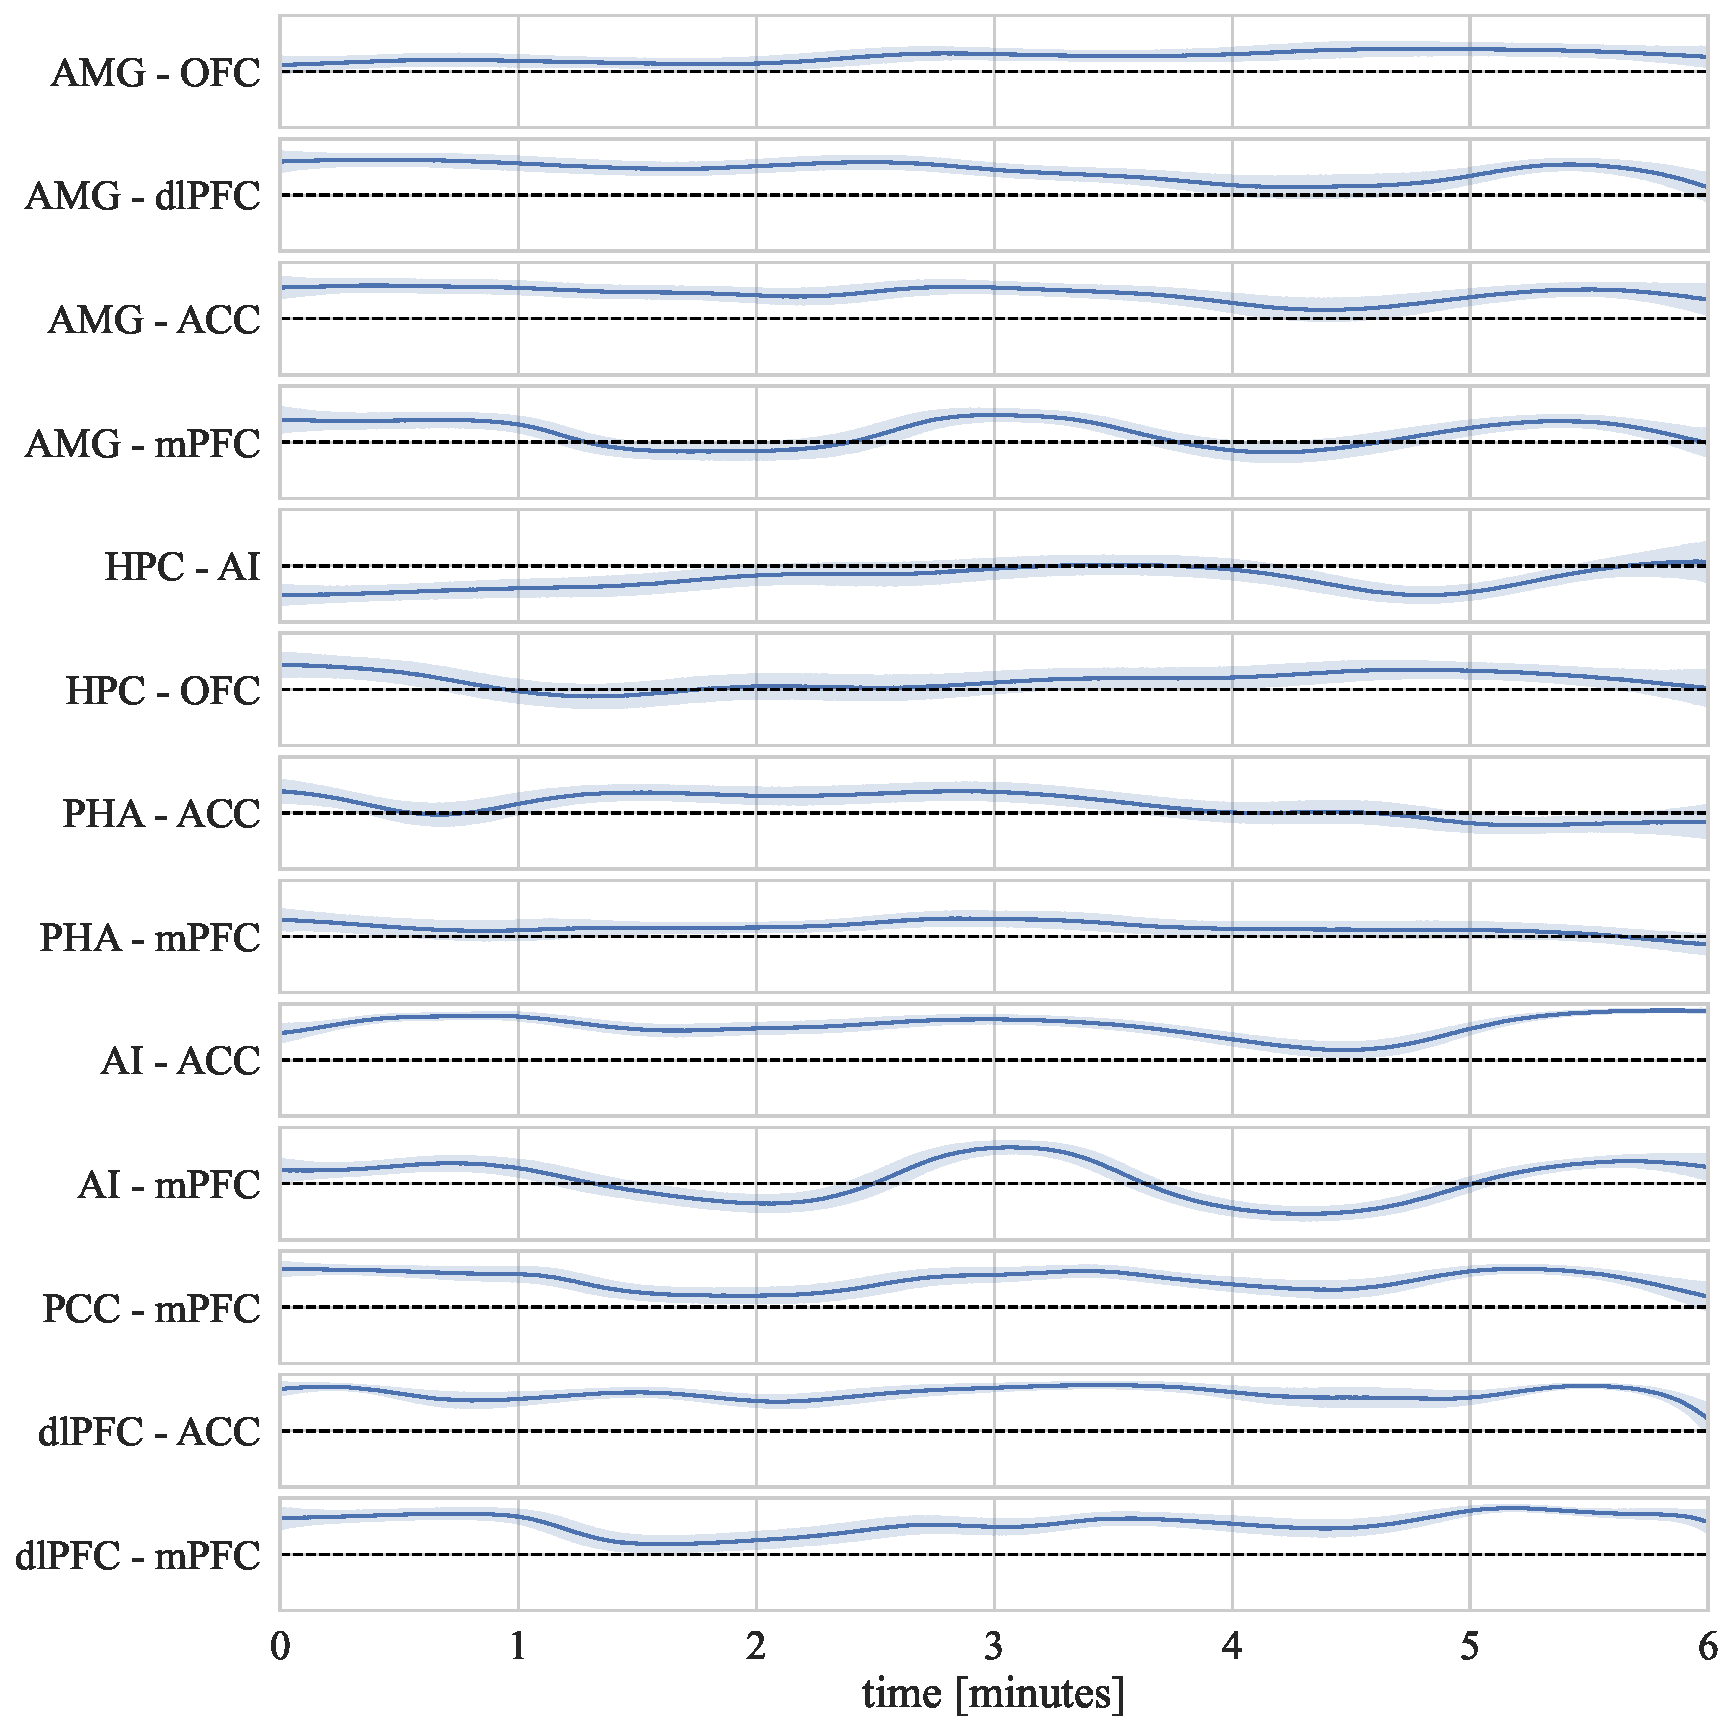
\includegraphics[width=0.95\textwidth]{fig/ukbiobank/TVFC_predictions/ROI/correlation_UKB1000211_TVFC_predictions}
  \caption{
    UK Biobank depression study TVFC estimates for a single (diagnosed lifetime occurrence depressed cohort) participant.
    Black dashed lines indicate uncorrelation.
  }\label{fig:ukbiobank-example-correlation-estimates-roi}
\end{figure}


Similarly, \cref{fig:ukbiobank-example-correlation-estimates-fn} shows \gls{tvfc} estimates for the same subject for all \gls{fn} interactions.
All \gls{fn} edges here show non-trivial time-varying structure and seem to capture the same global oscillatory structure.
%
However, interpretation remains difficult.
For example, what does the drop around the fourth minute mark in \gls{cen}--\gls{dmn} correlation mean?
Without further information, it is unclear whether this could indicate falling asleep, switching internal preoccupation, or any other speculation.


\begin{figure}[ht]
  \centering
  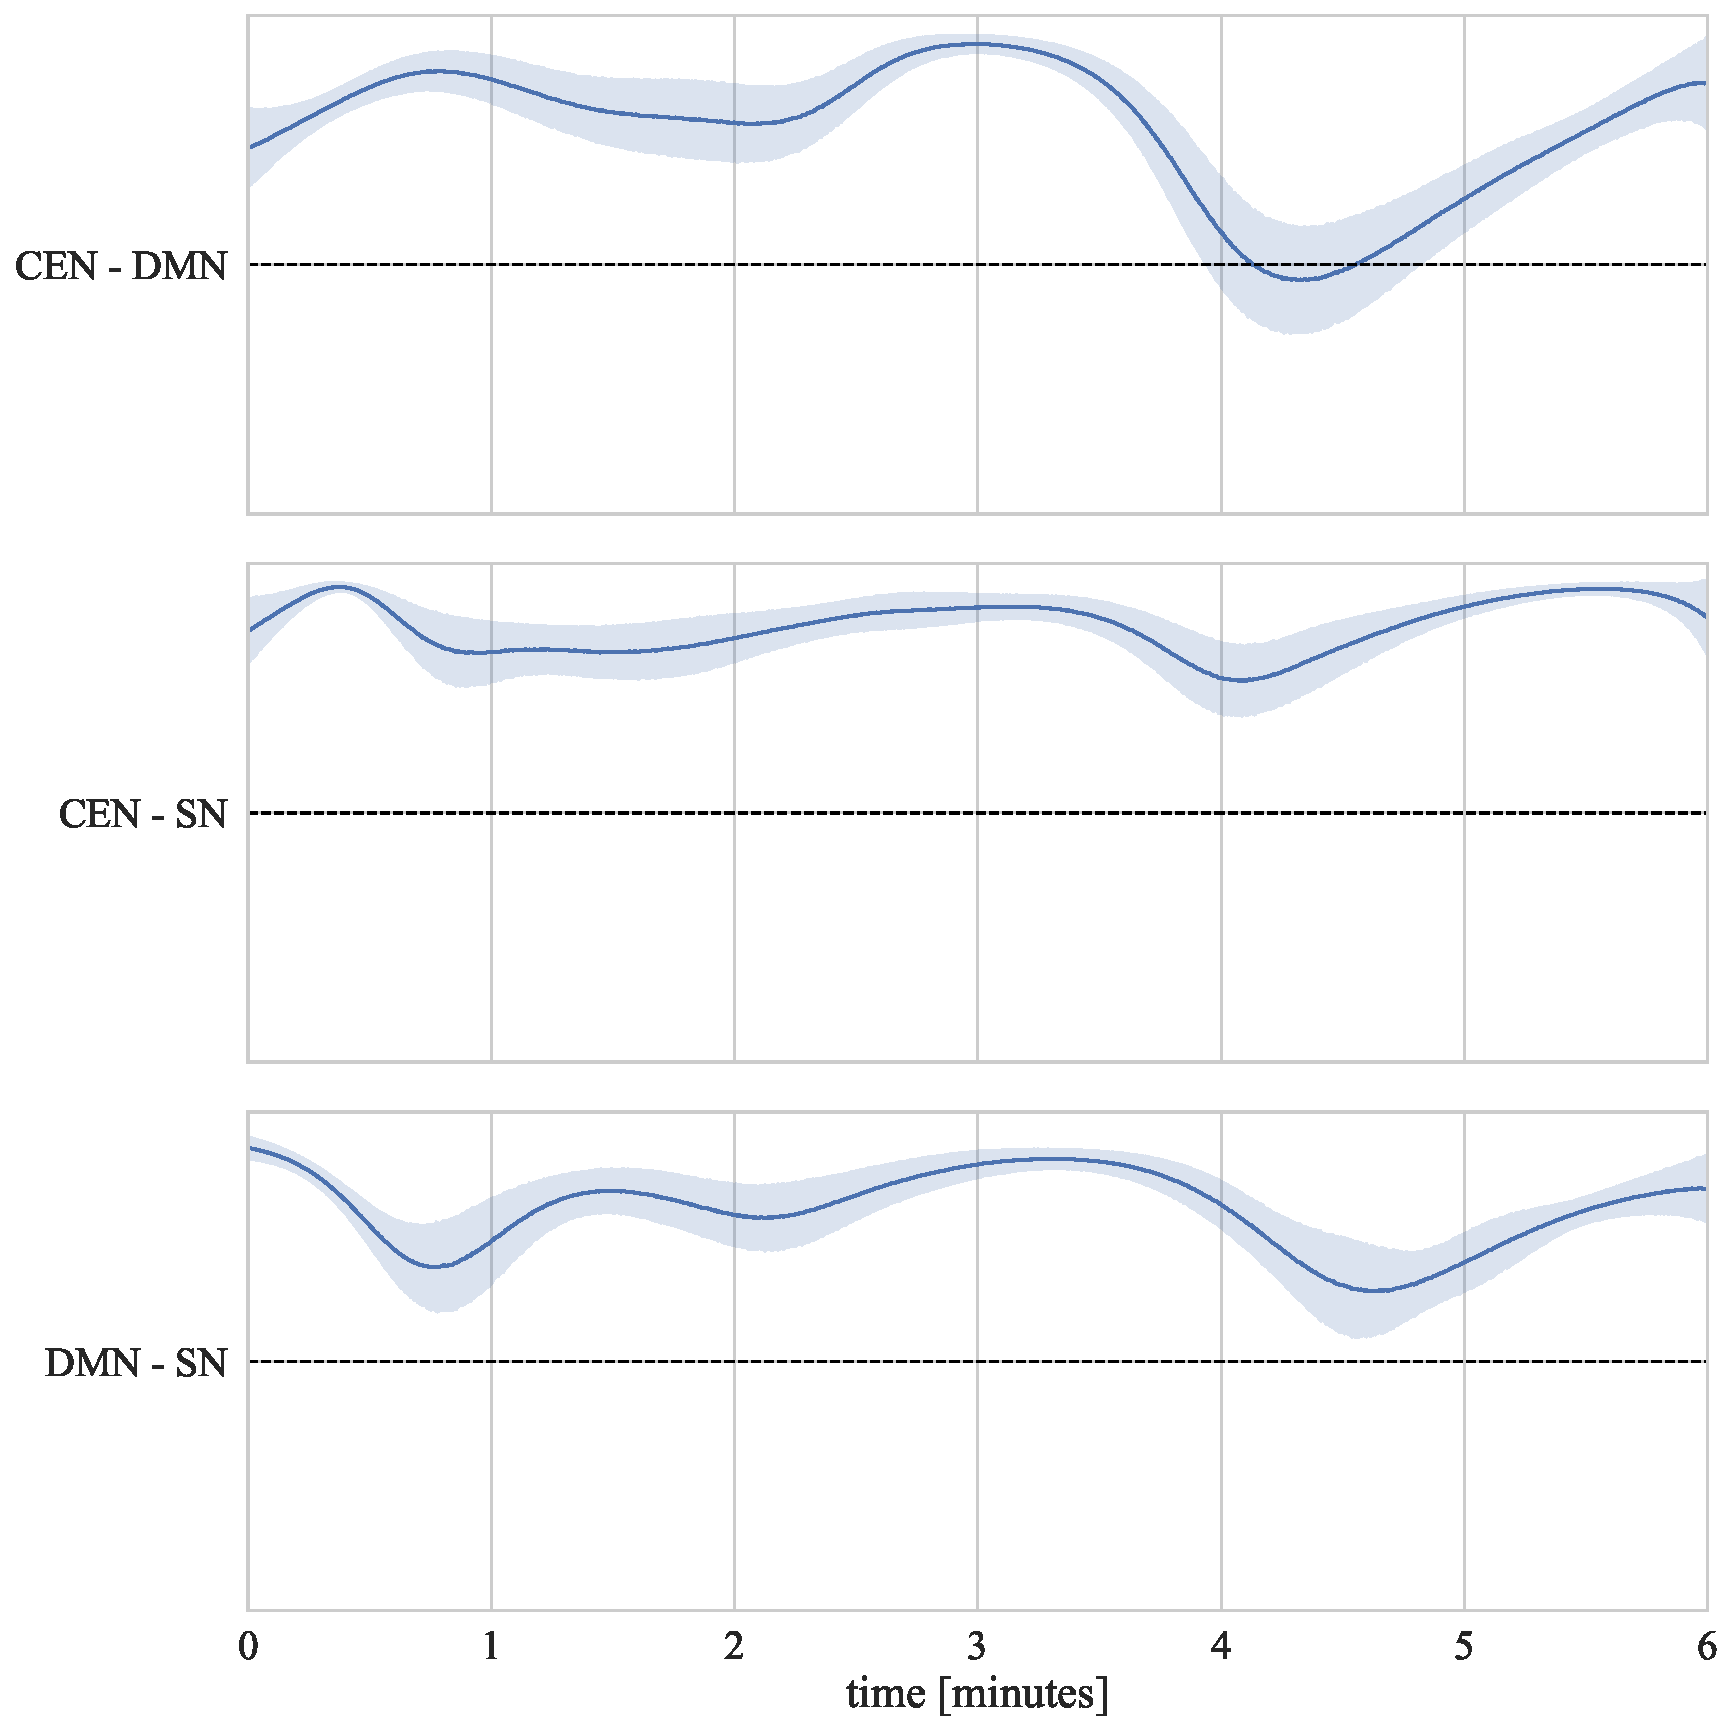
\includegraphics[width=0.85\textwidth]{fig/ukbiobank/TVFC_predictions/FN/correlation_UKB1000211_TVFC_predictions}
  \caption{
    UK Biobank depression study TVFC estimates for a single (diagnosed lifetime occurrence depressed cohort) participant for all interactions between the functional networks.
    Black dashed lines indicate uncorrelation.
  }\label{fig:ukbiobank-example-correlation-estimates-fn}
\end{figure}


Again, these are only estimates for a single subject.
Going forward, we rely on our \gls{tvfc} summary measures and brain state metrics to capture dynamics across the full cohorts.

%%
\subsection{Diagnosed lifetime occurrence}
%%

\Cref{fig:ukb-results-dlo-roi-cohort-comparison-full-wp} shows these summary measures for all edges between all brain \glspl{roi} for both cohorts.
The mean \gls{tvfc} estimates give an indication of population-level connectivity strengths.
No major differences can be seen at first here with the naked eye; as expected effect sizes are likely to be small.
In fact, these correlation matrices look similar across all phenotypes.
Therefore, the same results for the other three phenotypes are moved to \cref{fig:ukb-results-lo-roi-cohort-comparison-full-wp,fig:ukb-results-srds-roi-cohort-comparison-full-wp,fig:ukb-results-pgs-roi-cohort-comparison-full-wp}.
The \gls{amg} is most strongly connected to the \gls{hpc}, which is unsurprising as they are both part of the limbic system.


\begin{figure}[ht]
  \centering
  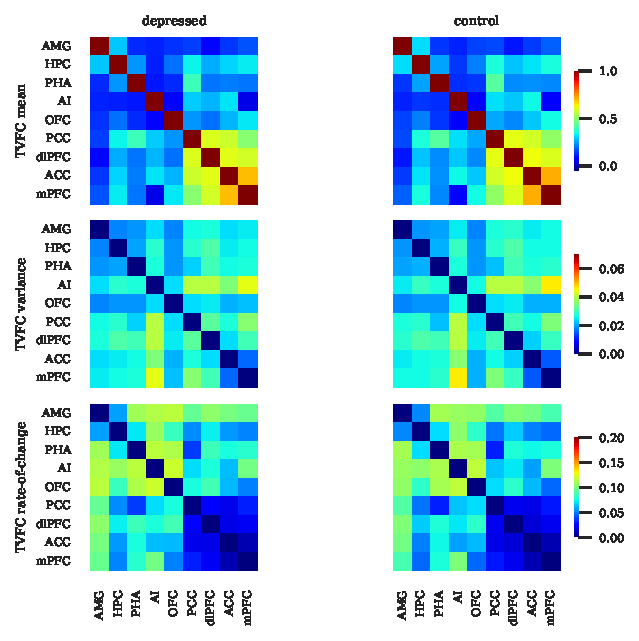
\includegraphics[width=0.9\textwidth]{fig/ukbiobank/TVFC_predictions_summaries/diagnosed_lifetime_occurrence/cohort_comparison/ROI/correlation_TVFC_estimates_SVWP_joint_joint}
  \caption{
    Diagnosed depression lifetime occurrence analysis - SVWP estimates.
    Mean over 620 subjects per cohort for all ROI edges, for three TVFC summary measures.
  }\label{fig:ukb-results-dlo-roi-cohort-comparison-full-wp}
\end{figure}


Next, we zoom in on the particular edges of interest.
Firstly, \cref{fig:ukb-results-dlo-roi-cohort-comparison-edges-of-interest-sfc} shows the \gls{sfc} estimates for these for both cohorts.
These estimates will be used as a reference later; \gls{tvfc} mean estimates should be similar.
As expected, strong coupling is found between prefrontal areas \gls{dlpfc}, \gls{acc}, and \gls{mpfc}, as well as \gls{pcc}--\gls{mpfc} (due to being the key components of the \gls{dmn}).
%
We find \emph{decreased} connectivity with \gls{mdd} across the board for all edges of interest.
This suggests some global association effect of a lifetime instance of \gls{mdd} on all brain region connections.
The largest effect size is found for the \gls{hpc}--\gls{ai} edge (Cohen~$d = 0.19$, $t(1235) = -3.32$, $p = .0047$) and the smallest for \gls{dlpfc}--\gls{mpfc} (Cohen~$d = 0.12$, $t(1228) = -2.10$, $p = .0393$).


\begin{figure}[t]
  \centering
  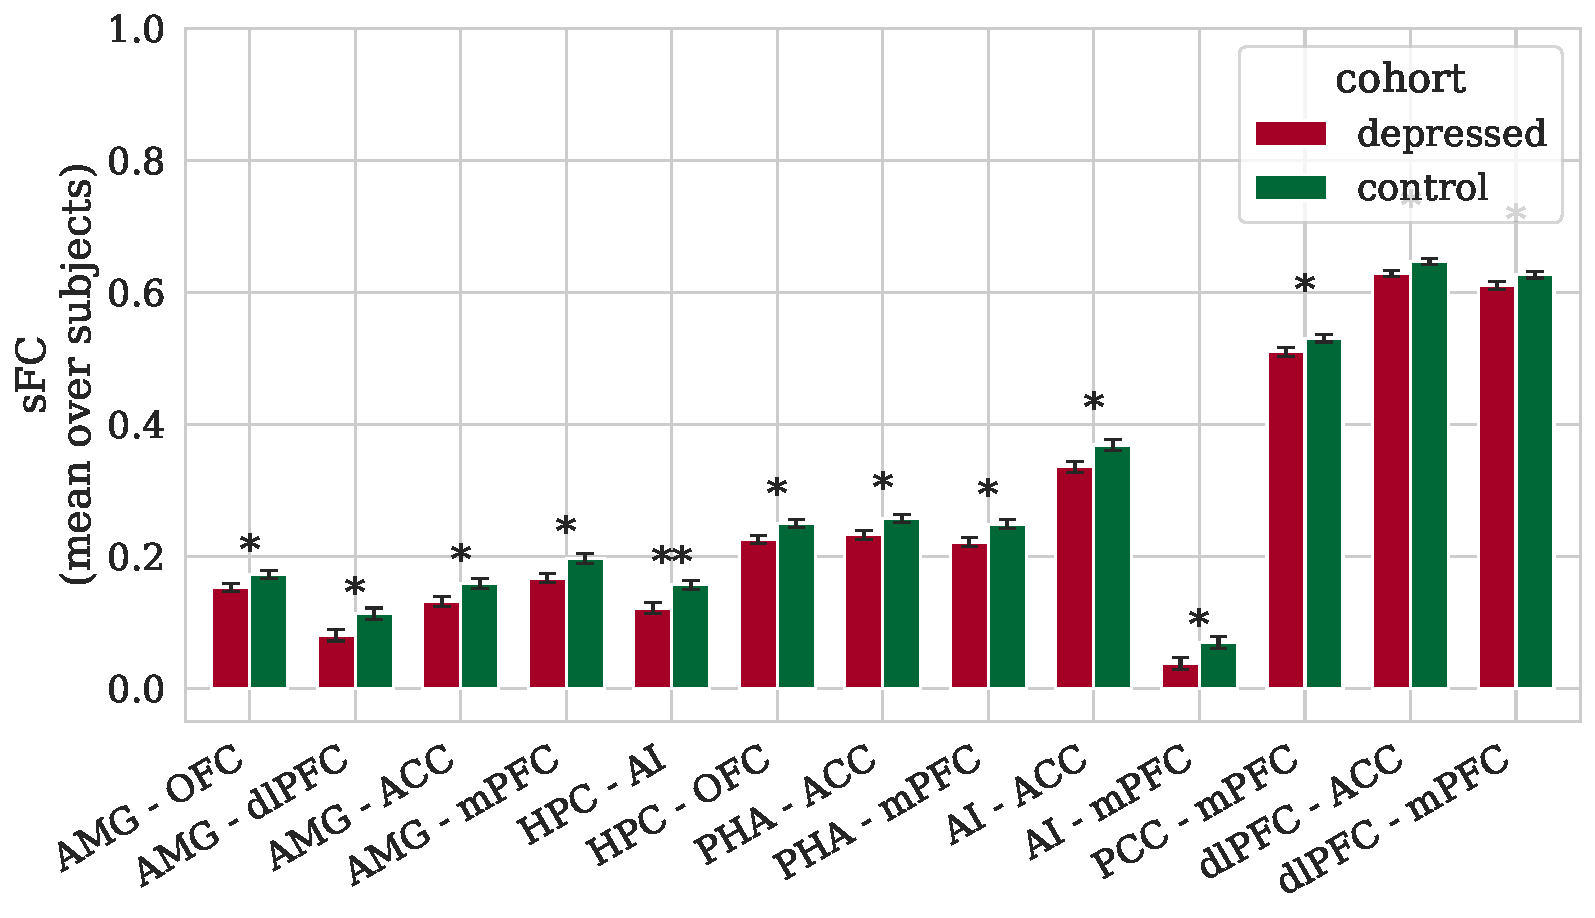
\includegraphics[width=0.85\textwidth]{fig/ukbiobank/TVFC_predictions_summaries/diagnosed_lifetime_occurrence/cohort_comparison/ROI/correlation_TVFC_mean_sFC_edges_of_interest}
  \caption{
    Diagnosed depression lifetime occurrence analysis - brain regions of interest - sFC estimates.
    Mean and standard error over 620 subjects per cohort for edges of interest.
    *: $p \leq .05$, **: $p \leq .01$.
  }\label{fig:ukb-results-dlo-roi-cohort-comparison-edges-of-interest-sfc}
\end{figure}


\Cref{fig:ukb-results-dlo-roi-cohort-comparison-edges-of-interest-wp} shows \gls{svwp} \gls{tvfc} estimates summary measures for the edges of interest between our brain regions of interest for both cohorts.
%
We find the same global decrease with \gls{mdd} in connectivity strength for all edges.
As expected, the mean \gls{tvfc} estimates are almost identical to the \gls{sfc} estimates.
However, significance and effect sizes are slightly different, with generally smaller $p$ values and larger Cohen~$d$ values found.
Here we find the smallest effect size for \gls{amg}--\gls{acc} (Cohen~$d = 0.12$, $t(1234) = -2.13$, $p = .0352$) and largest again for \gls{hpc}--\gls{ai} (Cohen~$d = 0.21$, $t(1235) = -3.61$, $p = .0019$).
%
For the variance summary measure, we find slight increases between prefrontal areas as well as decreases or no differences for all other edges.
However, none differ significantly across the cohorts.
The only edge here with a pre-\gls{mht} significant difference is \gls{dlpfc}--\gls{acc}.
%
For the rate-of-change summary measure, we see slightly increased values in the \gls{mdd} cohort for all edges except \gls{amg}--\gls{acc}.
We find significant increases for only two edges: \gls{hpc}--\gls{ofc} (Cohen~$d = 0.15$, $t(1020) = 2.57$, $p = .0458$) and \gls{dlpfc}--\gls{acc} (Cohen~$d = 0.16$, $t(1110) = 2.78$, $p = .0344$).
This finding is promising; finding cohort contrasts in \gls{tvfc} dynamics motivates the study thereof, beyond just \gls{sfc} analyses.
How could we interpret this finding for these two edges?
As we have learned from the subject measure prediction benchmark in the previous chapter (see \cref{fig:hcp-results-subject-measures-prediction}), the rate-of-change summary measure may be especially suitable for capturing subject characteristics related to language and memory.
Since we know the \gls{hpc} plays a key role in memory and cardinal depressive symptoms like rumination (obsessive and repetitive thoughts related to prior experiences), it is not surprising to find changes in this region with \gls{mdd}.\footnote{Such comparisons also demonstrate that benchmarking is not just about picking the best method. It helps us as a community to catalogue what features, representations, metrics, and/or constructs are useful, to what extent, and in what context~\parencite[see also][]{Voytek2022}.}


\begin{figure}[t]
  \centering
  \includegraphics[width=\textwidth]{fig/ukbiobank/TVFC_predictions_summaries/diagnosed_lifetime_occurrence/cohort_comparison/ROI/correlation_all_TVFC_summary_measures_SVWP_joint_edges_of_interest}
  \caption{
    Diagnosed depression lifetime occurrence analysis - brain regions of interest - SVWP estimates.
    Mean and standard error over 620 subjects per cohort for edges of interest for three TVFC summary measures.
    *: $p \leq .05$, **: $p \leq .01$.
  }\label{fig:ukb-results-dlo-roi-cohort-comparison-edges-of-interest-wp}
\end{figure}


\Cref{fig:ukb-results-dlo-fn-cohort-comparison-edges-of-interest-wp} shows \gls{tvfc} summary measures for all edges between our \glspl{fn} for both cohorts.
%
All estimate means (i.e.~\gls{sfc}) are \emph{reduced} in the \gls{mdd} cohort (Cohen~$d = 0.26, 0.31, 0.26$, respectively).
This echoes the global decreased connectivity strength effect found with the \gls{roi} analysis.
%
All \gls{tvfc} variances and rates-of-change are \emph{increased} with \gls{mdd}, but these differences are only significant with the latter (Cohen~$d = 0.25, 0.23, 0.21$, respectively).
The pre-\gls{mht} variances of \gls{cen}--\gls{sn} and \gls{dmn}--\gls{sn} are significantly increased, however.
Both the effect sizes and the statistical significance of these cohort contrast are much larger than with the \gls{roi} analysis.


\begin{figure}[ht]
  \centering
  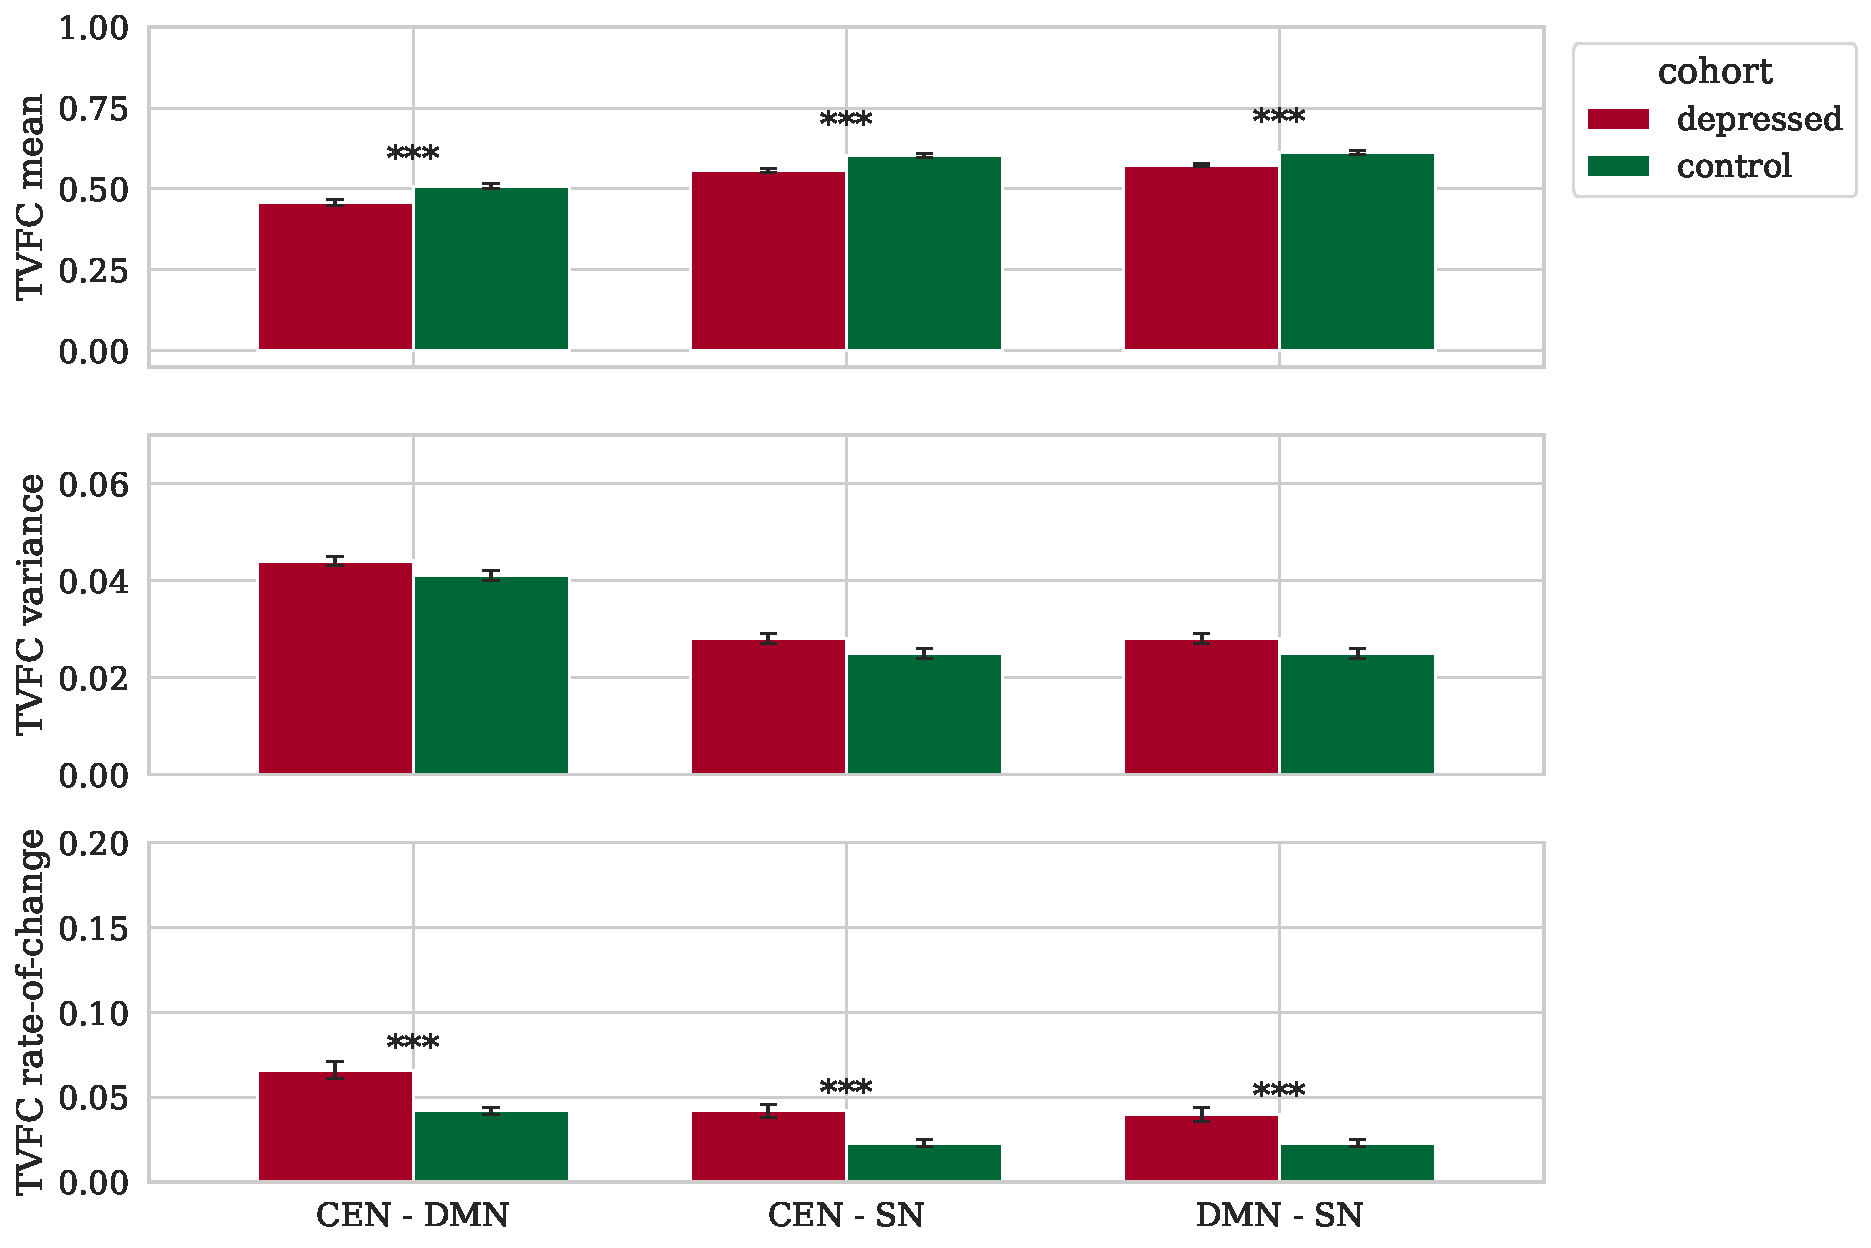
\includegraphics[width=0.7\textwidth]{fig/ukbiobank/TVFC_predictions_summaries/diagnosed_lifetime_occurrence/cohort_comparison/FN/correlation_all_TVFC_summary_measures_SVWP_joint_edges_of_interest}
  \caption{
    Diagnosed depression lifetime occurrence analysis - functional networks - SVWP estimates.
    Mean and standard error over 620 subjects per cohort for edges of interest for three TVFC summary measures.
    ***: $p \leq .001$.
  }\label{fig:ukb-results-dlo-fn-cohort-comparison-edges-of-interest-wp}
\end{figure}


Finally, compared to previous studies, this depression phenotype does not replicate many \gls{sfc} findings.
Many prior findings found \emph{increases} or \emph{specific} decreases in connectivity strength with \gls{mdd}.
We only find reduced connectivity strength across the board.

%%
\clearpage
\subsection{Self-reported lifetime occurrence}
%%

\Cref{fig:ukb-results-lo-roi-cohort-comparison-edges-of-interest-sfc} shows the \gls{sfc} estimates for the edges of interest for both cohorts.
These will be used as references again.
%
Interestingly, none of the edges bar \gls{hpc}--\gls{ai} (Cohen~$d = 0.14$) show any cohort contrast here.
This edge may be robustly affected by depression, as it also accounted for the smallest $p$-value and largest effect size among all edges in the previously studied depression phenotype.


\begin{figure}[h]
  \centering
  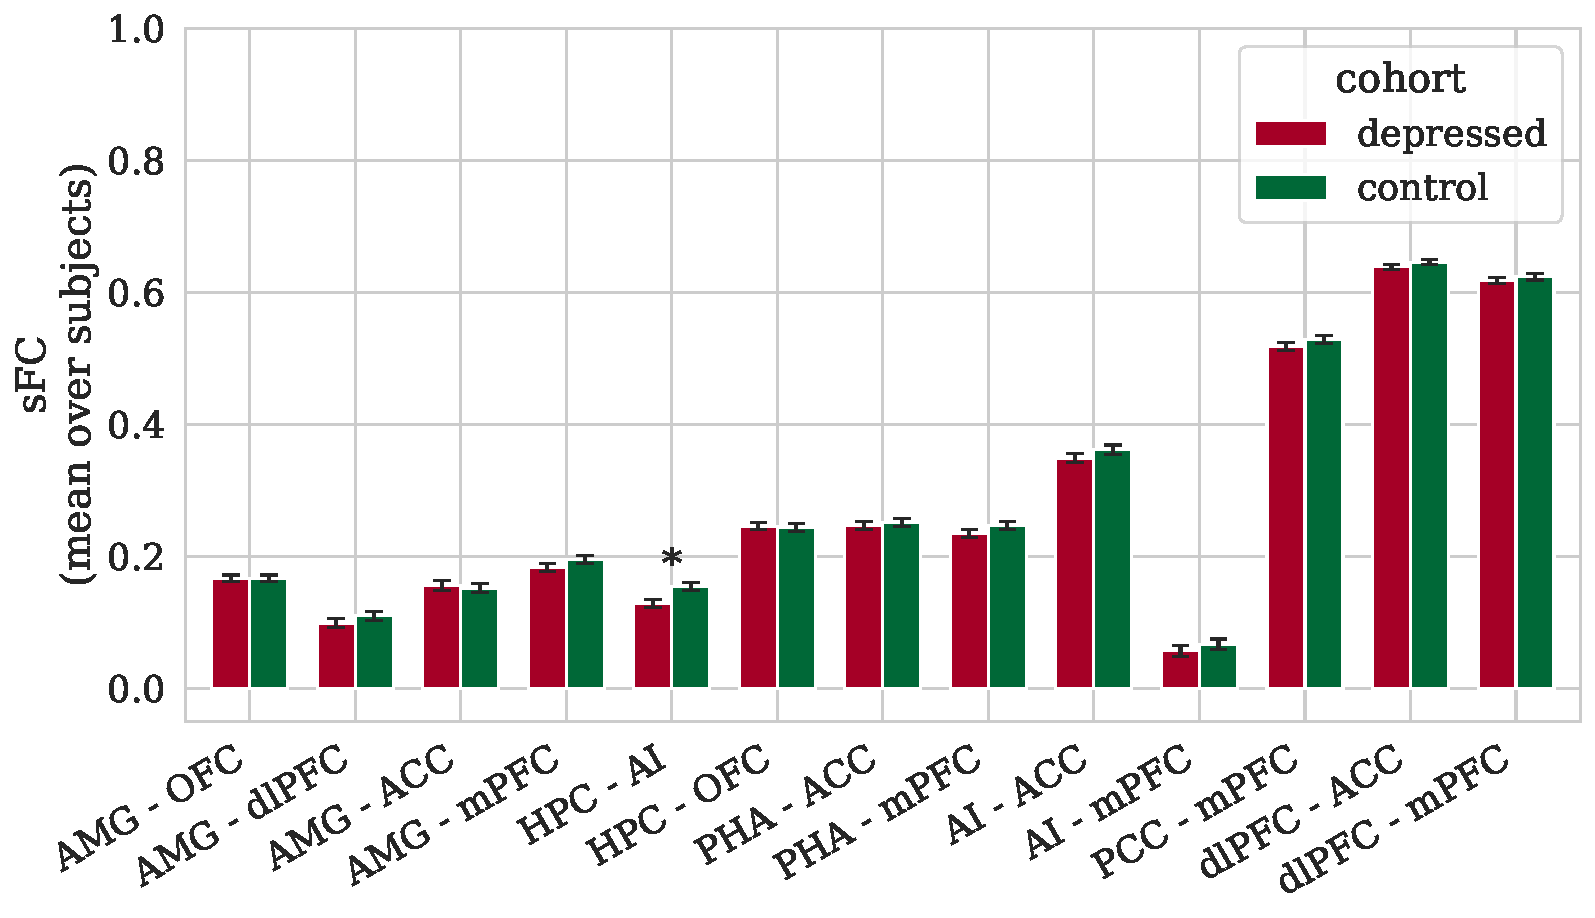
\includegraphics[width=0.85\textwidth]{fig/ukbiobank/TVFC_predictions_summaries/lifetime_occurrence/cohort_comparison/ROI/correlation_TVFC_mean_sFC_edges_of_interest}
  \caption{
    Self-reported depression lifetime occurrence analysis - brain regions of interest - sFC estimates.
    Mean and standard error over 808 subjects per cohort for edges of interest.
    *: $p \leq .05$.
  }\label{fig:ukb-results-lo-roi-cohort-comparison-edges-of-interest-sfc}
\end{figure}


\Cref{fig:ukb-results-lo-roi-cohort-comparison-edges-of-interest-wp} shows the \gls{roi} analysis \gls{svwp} \gls{tvfc} estimates cohort contrasts for the edges of interest.
%
The mean estimates again replicate the \gls{sfc} estimates.
There is only a single (static) edge that shows a significant contrast with this depression phenotype: the connection between the \gls{hpc} and the \gls{ai} (Cohen~$d = 0.15$).
So why would this edge be so relevant in depression?
Firstly, we can look at previous studies that found this edge to be involved with depression.
In fact, \textcite{Ellard2019} found the connection between \gls{ai} and limbic regions (including \gls{hpc} and caudate) to be affected in a related mood disorder: bipolar disorder.
Both insular and hippocampal gray matter volumes have also been observed to be lower in patients with \gls{mdd}~\parencite{Stratmann2014}.
In an \emph{effective} connectivity study, \textcite{Kandilarova2018} found that \gls{hpc} connectivity with other brain regions (including \gls{ai}) is strongly related to depression severity.
%
The absence of any significant cohort contrast for variance and rate-of-change summary measures is striking as well.
%
Further interpretation of why these results are so different from the ones found in the \emph{diagnosed} lifetime occurrence analysis will be discussed in \cref{subsec:variation-depression-phenotypes}.


\begin{figure}[t]
  \centering
  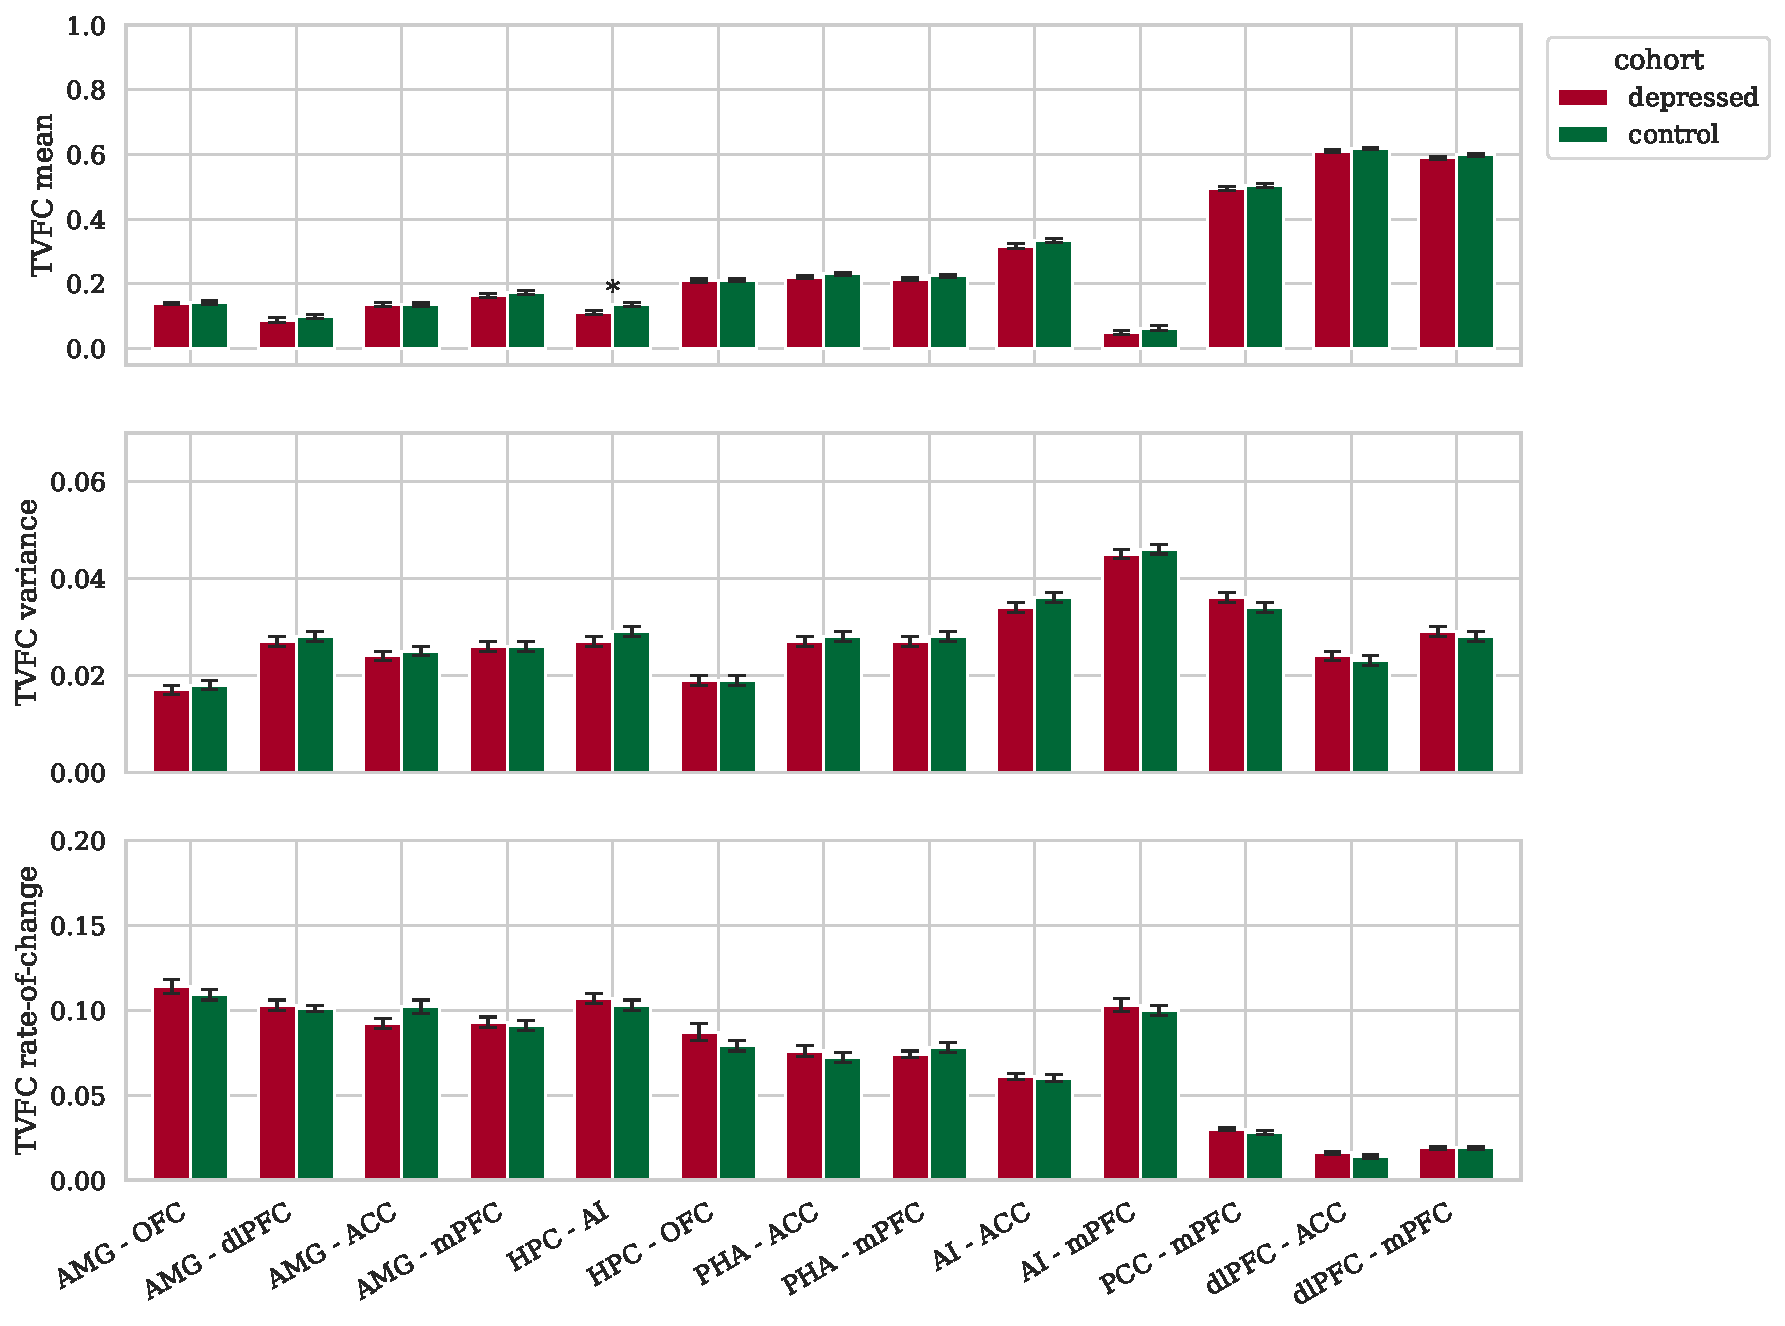
\includegraphics[width=\textwidth]{fig/ukbiobank/TVFC_predictions_summaries/lifetime_occurrence/cohort_comparison/ROI/correlation_all_TVFC_summary_measures_SVWP_joint_edges_of_interest}
  \caption{
    Self-reported depression lifetime occurrence analysis - brain regions of interest - SVWP estimates.
    Mean and standard error over 808 subjects per cohort for edges of interest for three TVFC summary measures.
    *: $p \leq .05$.
  }\label{fig:ukb-results-lo-roi-cohort-comparison-edges-of-interest-wp}
\end{figure}


Functional between-network connectivity estimates are shown in \cref{fig:ukb-results-lo-fn-cohort-comparison-edges-of-interest-wp}.
We find significant decreases in mean connectivity between \gls{cen} and \gls{dmn} (Cohen~$d = 0.12$) as well as \gls{cen} and \gls{sn} (Cohen~$d = 0.12$).
We find \emph{increases} for the same two edges for the rate-of-change summary measure (Cohen~$d = 0.12$ for both edges) with self-reported depression lifetime history.


\begin{figure}[h]
  \centering
  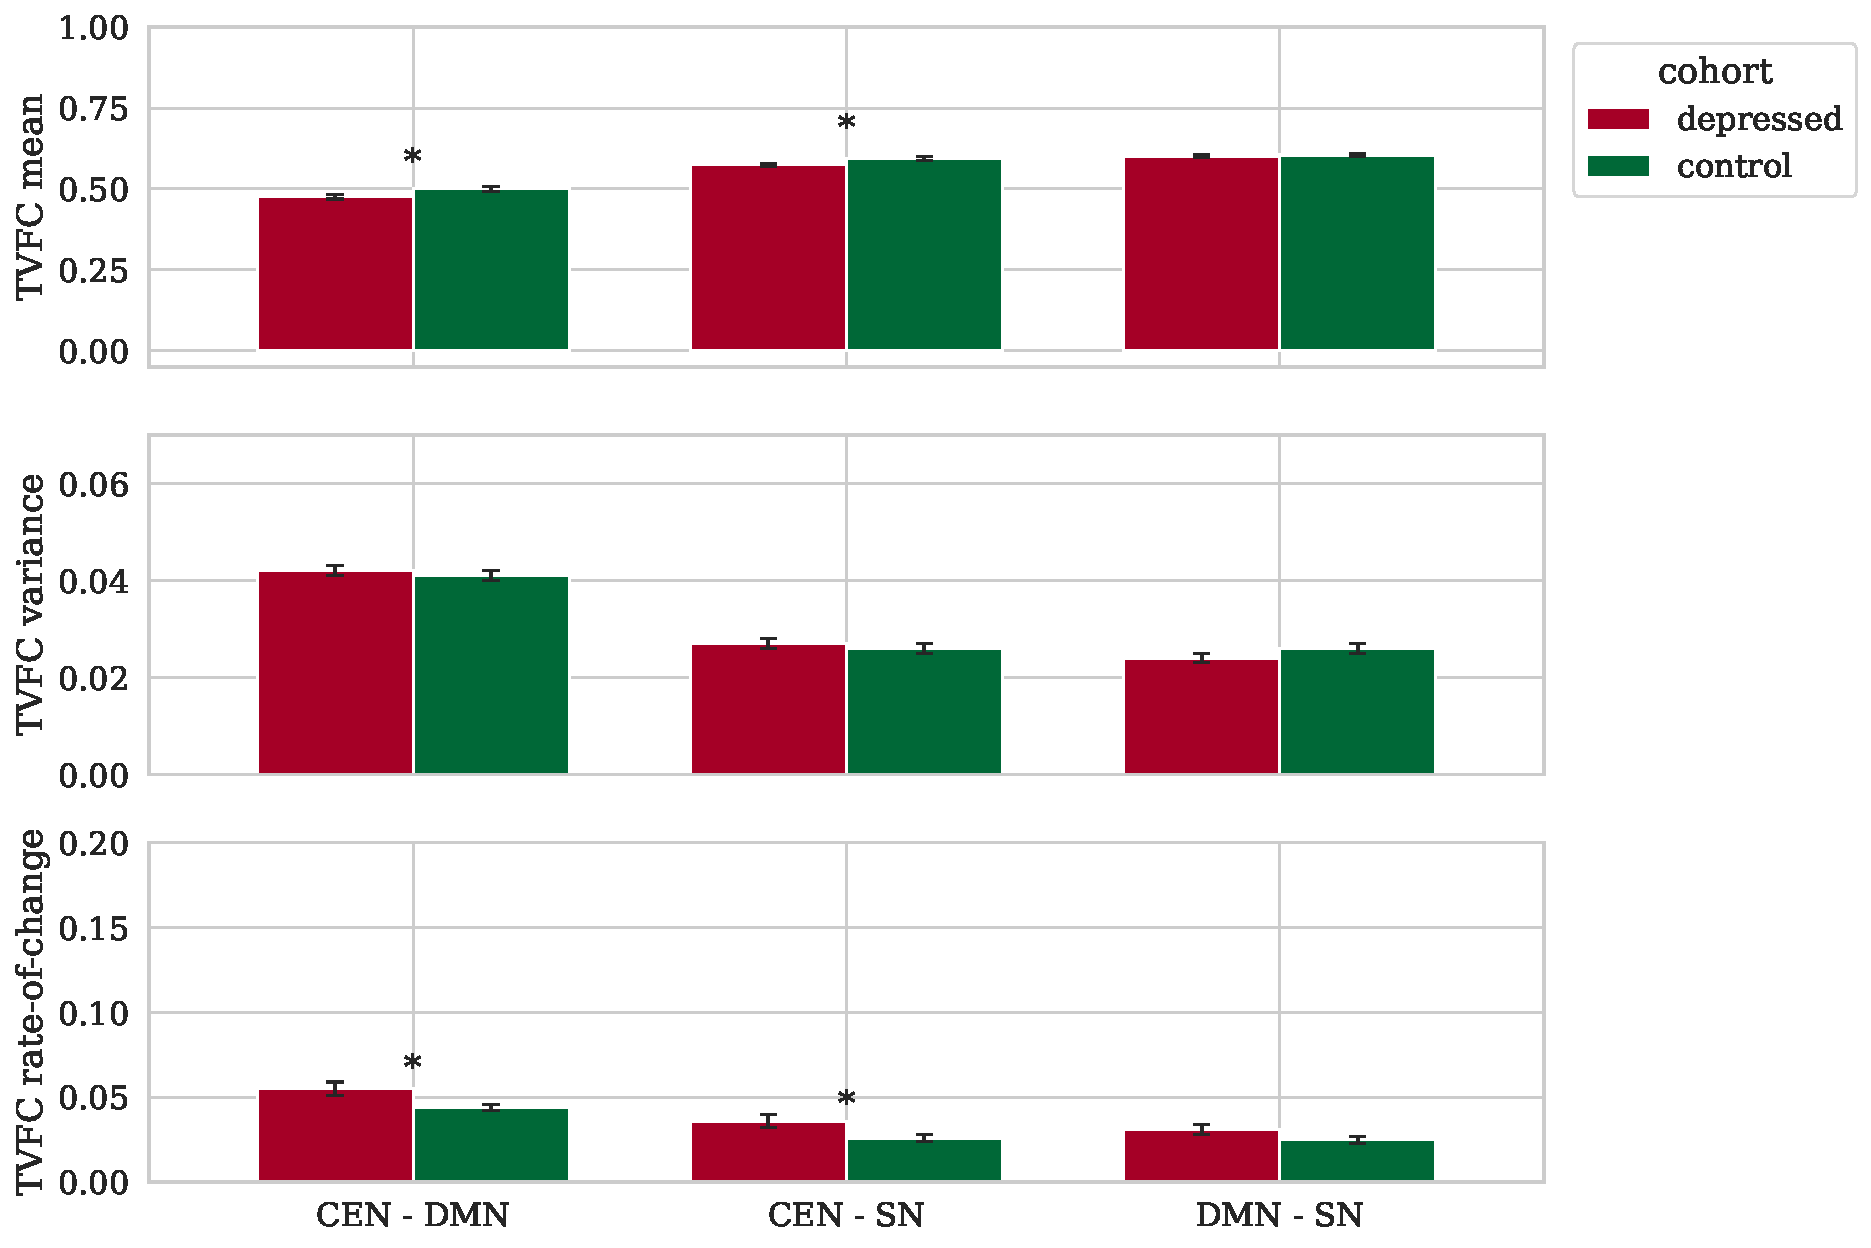
\includegraphics[width=0.7\textwidth]{fig/ukbiobank/TVFC_predictions_summaries/lifetime_occurrence/cohort_comparison/FN/correlation_all_TVFC_summary_measures_SVWP_joint_edges_of_interest}
  \caption{
    Self-reported depression lifetime occurrence analysis - functional networks - SVWP estimates.
    Mean and standard error over 808 subjects per cohort for edges of interest for three TVFC summary measures.
    *: $p \leq .05$.
  }\label{fig:ukb-results-lo-fn-cohort-comparison-edges-of-interest-wp}
\end{figure}


%%
\clearpage
\subsection{Self-reported depressed state}
%%

\Cref{fig:ukb-results-srds-roi-cohort-comparison-edges-of-interest-sfc} shows the \gls{sfc} estimates for this depression phenotype.
The results are, again, distinct from the previous two depression phenotypes.
%
However, we do see reduced connectivity again across the board for all edges.
These decreases are significant for most edges: \gls{amg}--\gls{mpfc} (Cohen~$d = 0.10$), \gls{amg}--\gls{ofc} (Cohen~$d = 0.10$), \gls{hpc}--\gls{ofc} (Cohen~$d = 0.10$), \gls{hpc}--\gls{ai} (Cohen~$d = 0.15$), \gls{pha}--\gls{acc} (Cohen~$d = 0.11$), \gls{pha}--\gls{mpfc} (Cohen~$d = 0.12$), \gls{ai}--\gls{acc} (Cohen~$d = 0.10$), \gls{ai}--\gls{mpfc} (Cohen~$d = 0.09$), and \gls{dlpfc}--\gls{acc} (Cohen~$d = 0.10$).
Again, we find the largest effect size for the \gls{hpc}--\gls{ai} edge.


\begin{figure}[h]
  \centering
  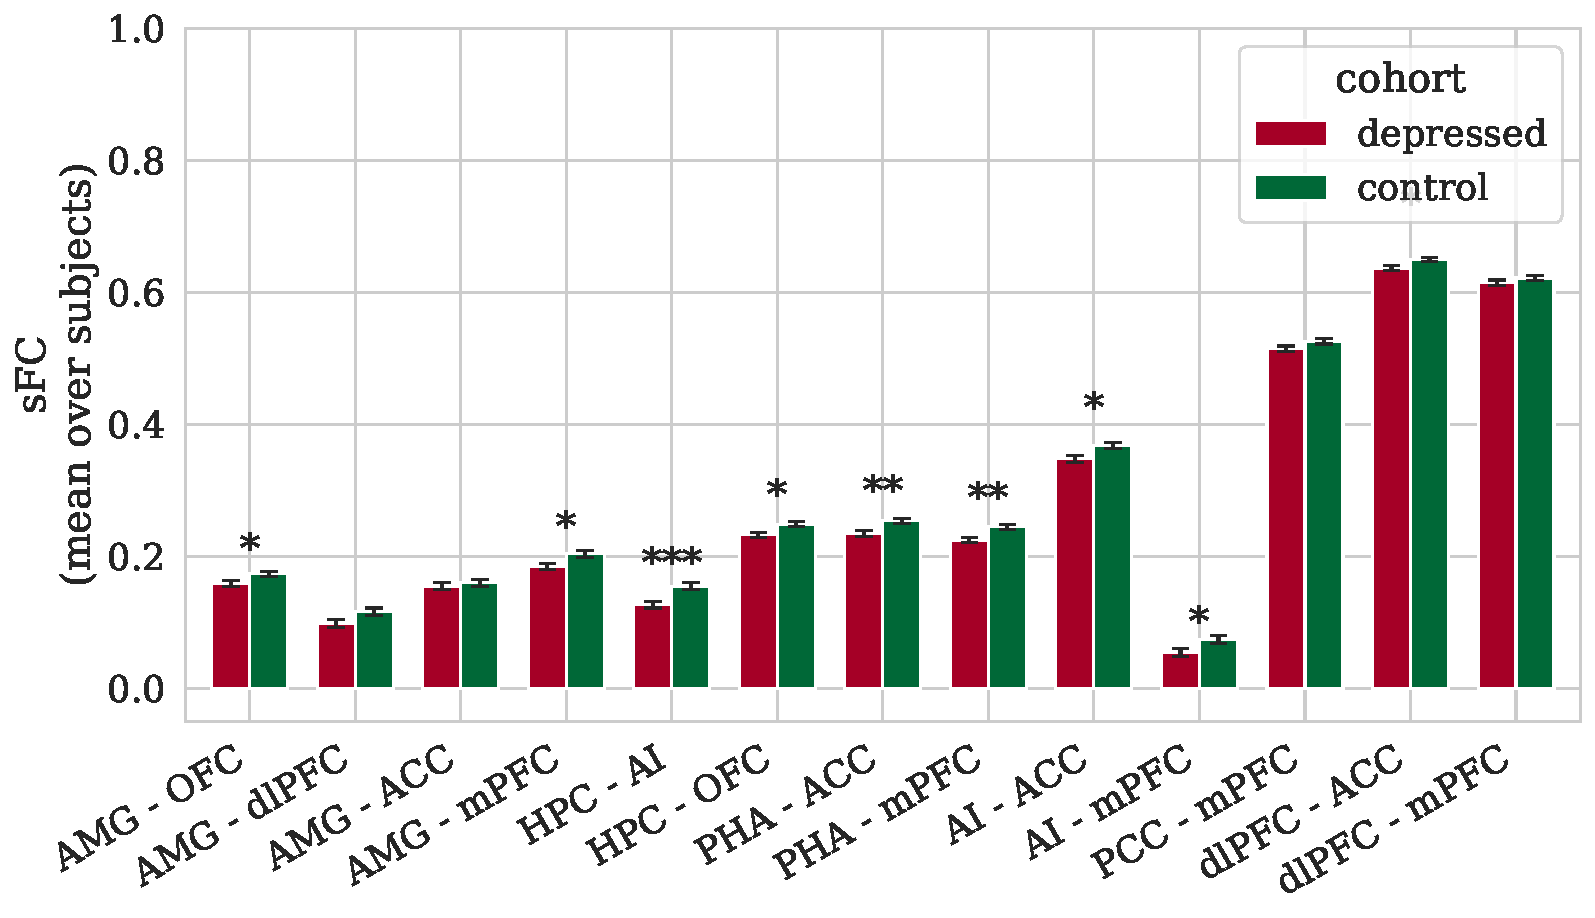
\includegraphics[width=0.85\textwidth]{fig/ukbiobank/TVFC_predictions_summaries/self_reported_depression_state/cohort_comparison/ROI/correlation_TVFC_mean_sFC_edges_of_interest}
  \caption{
    Self-reported depressed state analysis - brain regions of interest - sFC estimates.
    Mean and standard error over 1,411 subjects per cohort for edges of interest.
    *: $p \leq .05$, **: $p \leq .01$, ***: $p \leq .001$.
  }\label{fig:ukb-results-srds-roi-cohort-comparison-edges-of-interest-sfc}
\end{figure}


\Cref{fig:ukb-results-srds-roi-cohort-comparison-edges-of-interest-wp} shows the \gls{svwp} \gls{tvfc} estimates for this depression phenotype.
%
The estimate means broadly correspond with the \gls{sfc}.
However, here we find additional significant decreases for three additional edges: \gls{amg}--\gls{dlpfc} (Cohen~$d = 0.08$), \gls{dlpfc}--\gls{mpfc} (Cohen~$d = 0.08$), and \gls{pcc}--\gls{mpfc} (Cohen~$d = 0.09$).
%
In terms of \gls{tvfc} variance, we find increases with depression for the edges between prefrontal areas and decreases for all other edges.
However, none of these are significant, even before \gls{mht}, except for \gls{dlpfc}--\gls{acc}.
%
For \gls{tvfc} rate-of-change, we find increases for all edges, but none are significant again.
Three edges were significantly different across cohorts before \gls{mht}: \gls{amg}--\gls{mpfc}, \gls{amg}--\gls{ofc}, and \gls{dlpfc}--\gls{acc}.


\begin{figure}[h]
  \centering
  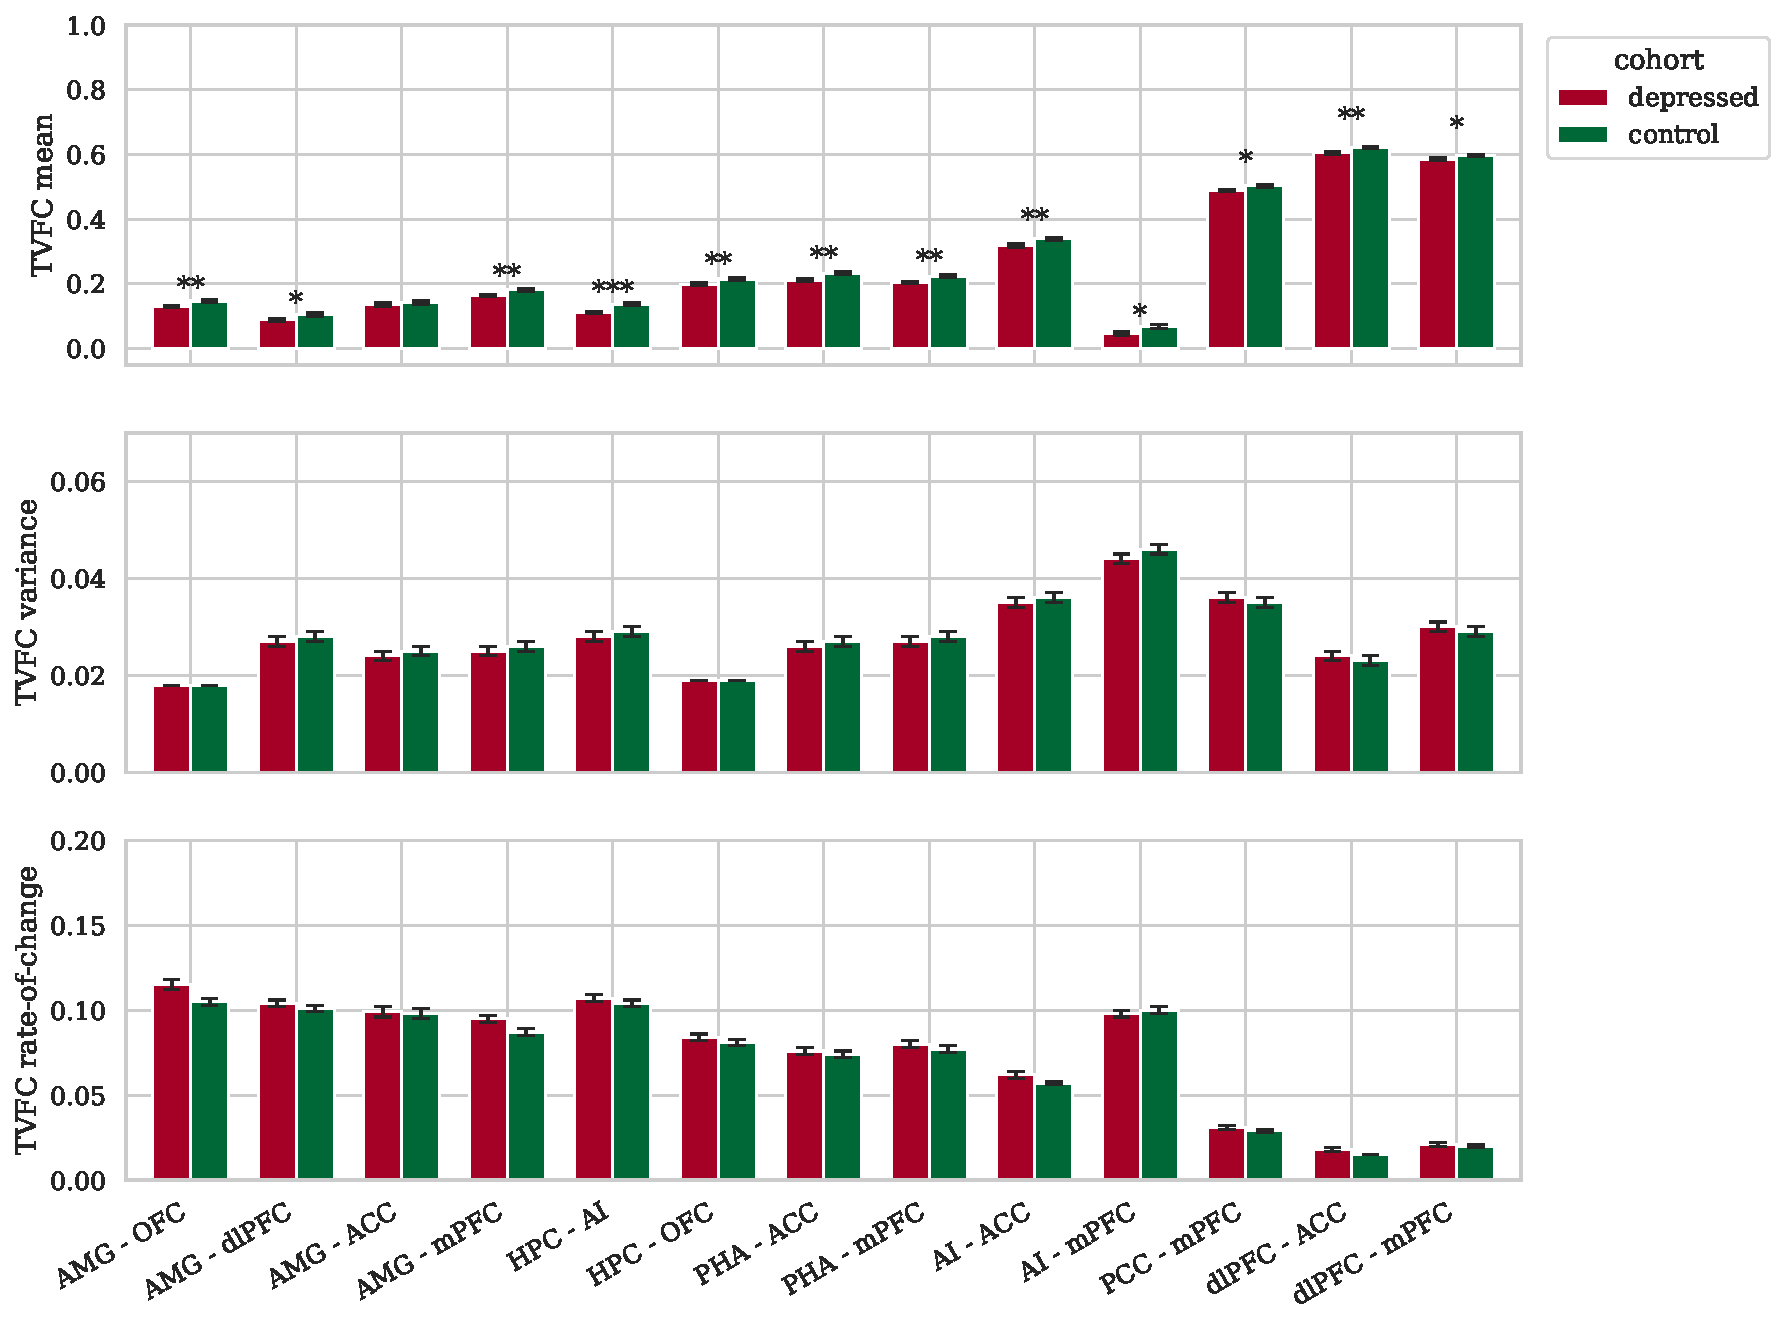
\includegraphics[width=\textwidth]{fig/ukbiobank/TVFC_predictions_summaries/self_reported_depression_state/cohort_comparison/ROI/correlation_all_TVFC_summary_measures_SVWP_joint_edges_of_interest}
  \caption{
    Self-reported depressed state analysis - brain regions of interest - SVWP estimates.
    Mean and standard error over 1,411 subjects per cohort for edges of interest for three TVFC summary measures.
    *: $p \leq .05$, **: $p \leq .01$, ***: $p \leq .001$.
  }\label{fig:ukb-results-srds-roi-cohort-comparison-edges-of-interest-wp}
\end{figure}


\Cref{fig:ukb-results-srds-fn-cohort-comparison-edges-of-interest-wp} shows the \gls{tvfc} estimates for the \glspl{fn}.
We find the same general trends as for the diagnosed lifetime occurrence phenotype here.
Decreased connectivity strength is found between all three networks (Cohen~$d = 0.15, 0.13, 0.13$, respectively.)
%
No significant contrasts in \gls{tvfc} variance are found.
Increases in \gls{tvfc} rate-of-change are found for all three networks (Cohen~$d = 0.12, 0.11, 0.11$, respectively).


\begin{figure}[h]
  \centering
  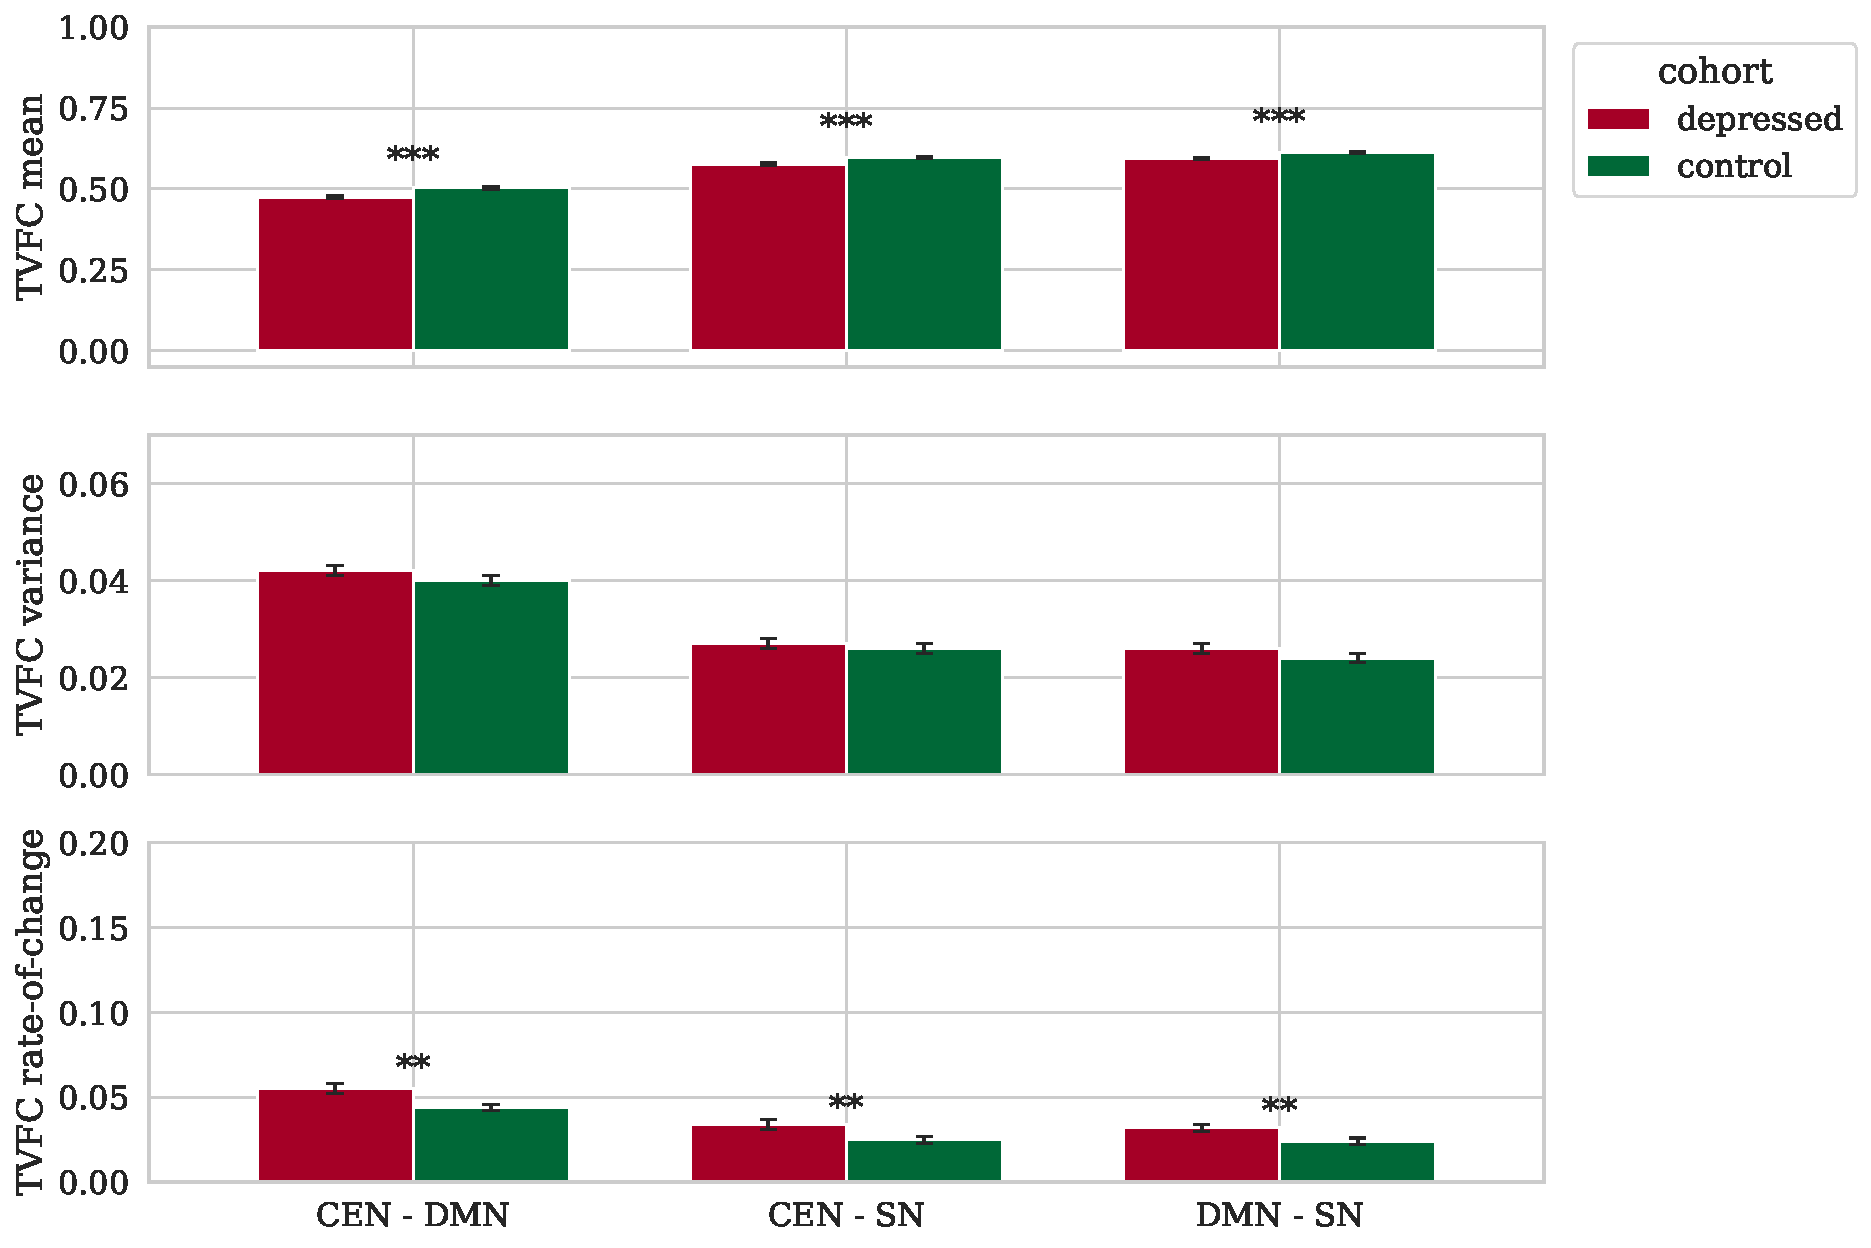
\includegraphics[width=0.7\textwidth]{fig/ukbiobank/TVFC_predictions_summaries/self_reported_depression_state/cohort_comparison/FN/correlation_all_TVFC_summary_measures_SVWP_joint_edges_of_interest}
  \caption{
    Self-reported depressed state analysis - functional networks - SVWP estimates.
    Mean and standard error over 1,411 subjects per cohort for edges of interest for three TVFC summary measures.
    *: $p \leq .05$, **: $p \leq .01$, ***: $p \leq .001$.
  }\label{fig:ukb-results-srds-fn-cohort-comparison-edges-of-interest-wp}
\end{figure}


%%
\clearpage
\subsection{Polygenic risk scores}
%%

\Cref{fig:ukb-results-pgs-roi-cohort-comparison-edges-of-interest-sfc} shows the \gls{sfc} cohort contrasts for only the edges of interest.
We generally do not find the same effects as with the other depression phenotypes.
In fact, we do not find \emph{any} contrasts between the cohorts for the static case in this depression phenotype.


\begin{figure}[h]
  \centering
  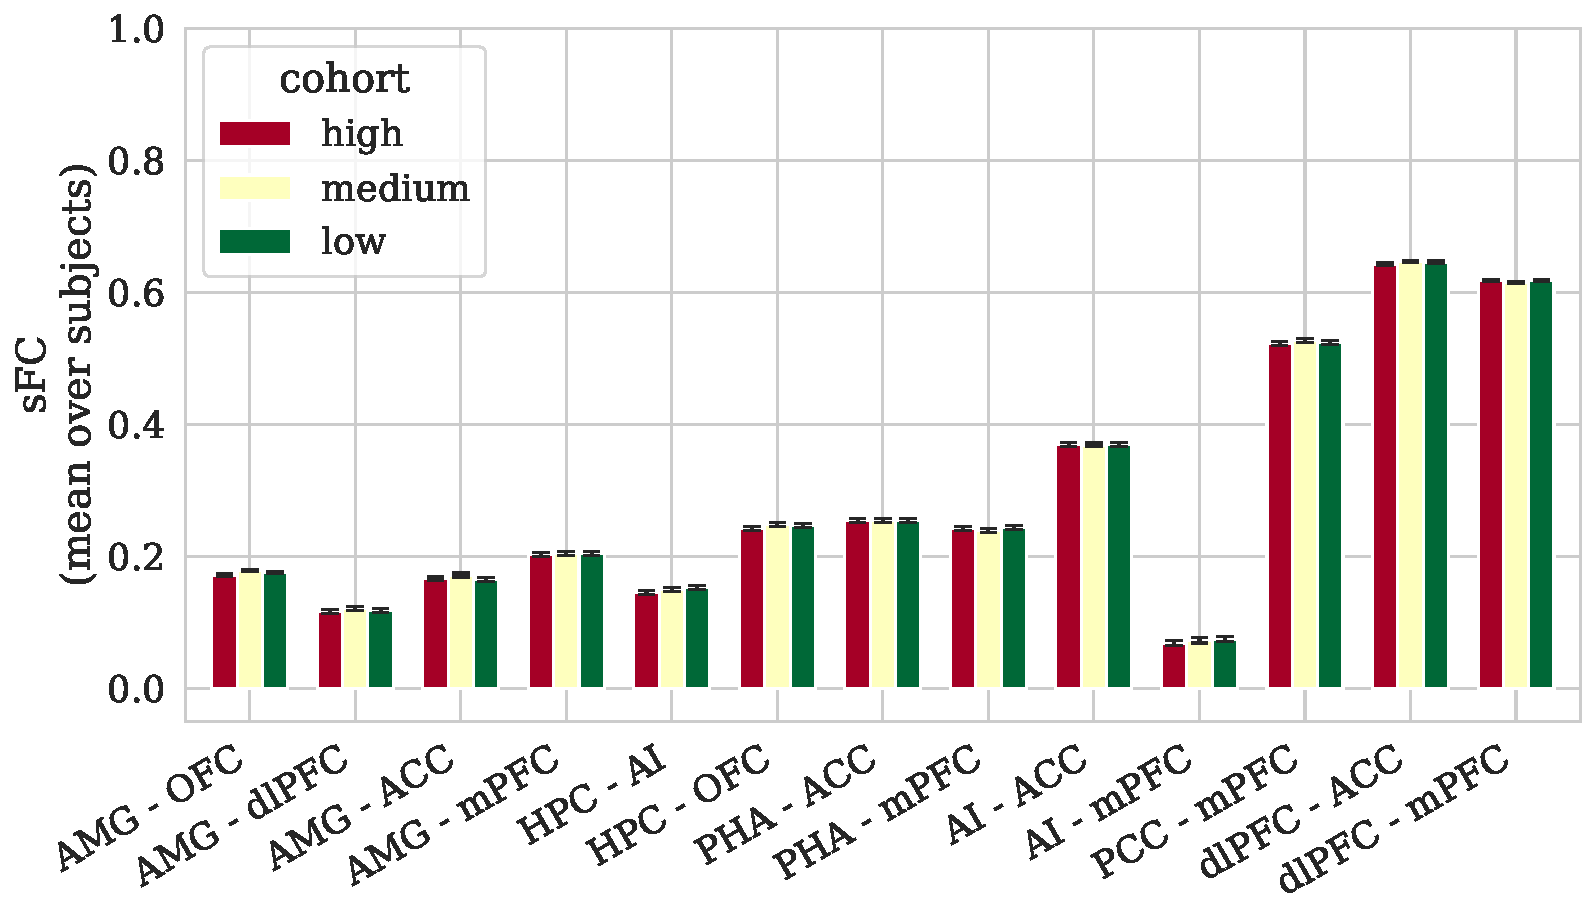
\includegraphics[width=0.85\textwidth]{fig/ukbiobank/TVFC_predictions_summaries/pgs/cohort_comparison/ROI/correlation_TVFC_mean_sFC_edges_of_interest}
  \caption{
    Polygenic risk scores analysis - brain regions of interest - sFC estimates.
    Mean and standard error over 3,775 subjects per cohort for edges of interest.
  }\label{fig:ukb-results-pgs-roi-cohort-comparison-edges-of-interest-sfc}
\end{figure}


\Cref{fig:ukb-results-pgs-roi-cohort-comparison-edges-of-interest-wp} shows the \gls{roi} cohort contrasts for the \gls{svwp} estimates.
None of the estimate means differ across cohorts.
None of the \gls{tvfc} variances are different across cohorts either (although \gls{amg}--\gls{dlpfc} variance is pre-\gls{mht} significantly higher in the high risk cohort).
None of the rate-of-change summary measures are different across cohorts either.


\begin{figure}[h]
  \centering
  \includegraphics[width=\textwidth]{fig/ukbiobank/TVFC_predictions_summaries/pgs/cohort_comparison/ROI/correlation_all_TVFC_summary_measures_SVWP_joint_edges_of_interest}
  \caption{
    Polygenic risk scores analysis - brain regions of interest - SVWP estimates.
    Mean and standard error over 3,775 subjects per cohort for edges of interest for three TVFC summary measures.
  }\label{fig:ukb-results-pgs-roi-cohort-comparison-edges-of-interest-wp}
\end{figure}


These findings are replicated in the \gls{fn} analysis, shown in \cref{fig:ukb-results-pgs-fn-cohort-comparison-edges-of-interest-wp}.


\begin{figure}[h]
  \centering
  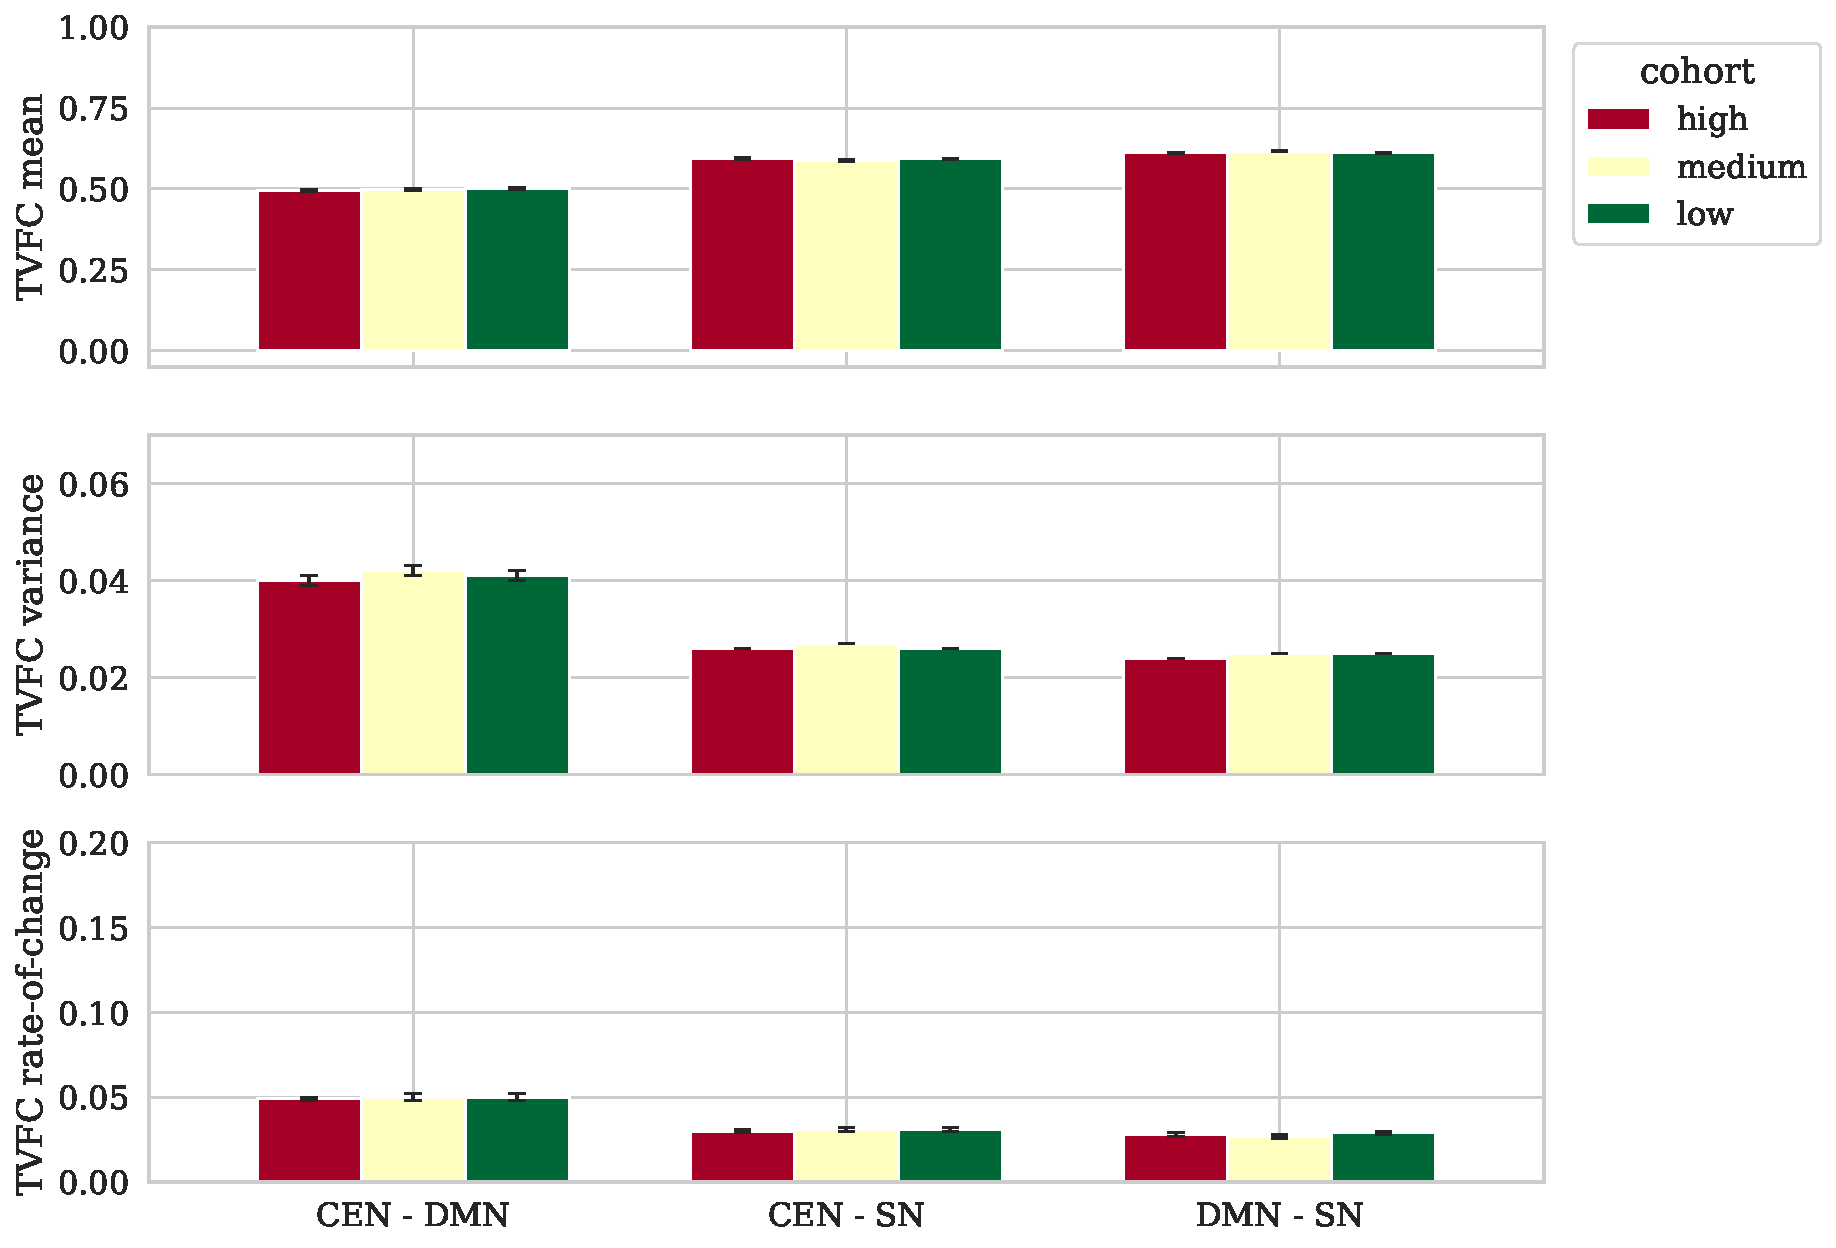
\includegraphics[width=0.7\textwidth]{fig/ukbiobank/TVFC_predictions_summaries/pgs/cohort_comparison/FN/correlation_all_TVFC_summary_measures_SVWP_joint_edges_of_interest}
  \caption{
    Polygenic risk scores analysis - functional networks - SVWP estimates.
    Mean and standard error over 3,775 subjects per cohort for edges of interest for three TVFC summary measures.
  }\label{fig:ukb-results-pgs-fn-cohort-comparison-edges-of-interest-wp}
\end{figure}


The \gls{prs} results suggest that genetic risk is not associated with differences in \gls{tvfc}.
We will return to this in the later discussion of results.

%%
\clearpage
\subsection{Brain states analysis}
%%

The extracted $k = 4$ brain states (as explicitly defined in \cref{subsec:brain-states}) are shown in \cref{fig:ukb-results-brain-states-dlo,fig:ukb-results-brain-states-srlo,fig:ukb-results-brain-states-srds} for the first three depression phenotypes.
The \gls{prs} phenotype is excluded here, as we found no cohort contrasts in the previous analysis.

Interestingly, the brain states extracted across the analysis types are almost identical.
All brain states have strong within-\gls{pfc} connectivity and connectivity between \gls{pha} and the \gls{pcc}.
%
Brain state~1 is characterized by weaker connectivity throughout, but especially within the \gls{pfc}.
%
Brain state~2 is characterized by especially stronger connectivity between the \gls{hpc} and prefrontal areas and between prefrontal areas themselves (compared to the first brain state and including within-\gls{dmn} connectivity).
The connectivity between the \gls{ai} and prefrontal areas is even weaker than found in the first brain state.
%
Brain state~3 is characterized by particularly \emph{strong} connectivity between the \gls{ai} and prefrontal areas.
%
Brain state~4 is characterized by overall higher connectivity between all \glspl{roi}.


\begin{figure}[ht]
  \centering
  \subcaptionbox{Diagnosed lifetime occurrence\label{fig:ukb-results-brain-states-dlo}}{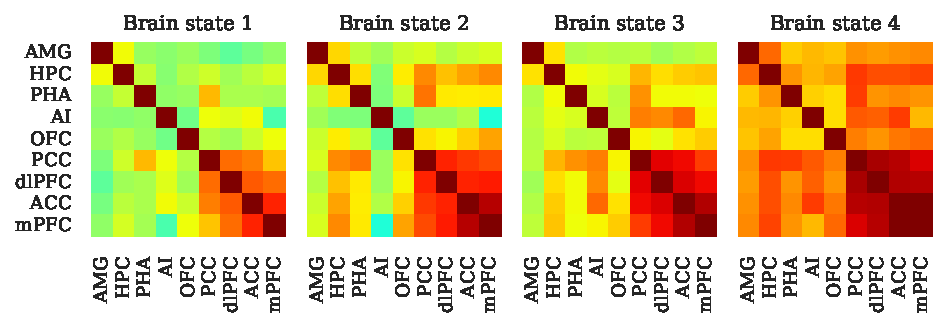
\includegraphics[width=\textwidth]{fig/ukbiobank/brain_states/diagnosed_lifetime_occurrence_brain_states_SVWP_joint_k04}}
  \subcaptionbox{Self-reported lifetime occurrence\label{fig:ukb-results-brain-states-srlo}}{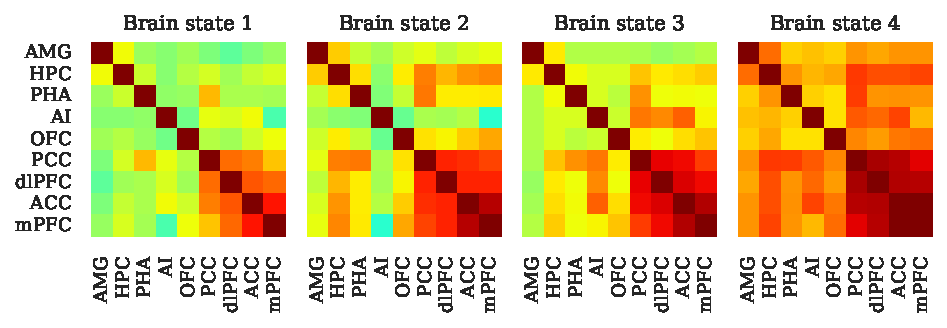
\includegraphics[width=\textwidth]{fig/ukbiobank/brain_states/lifetime_occurrence_brain_states_SVWP_joint_k04}}
  \subcaptionbox{Self-reported depressed state\label{fig:ukb-results-brain-states-srds}}{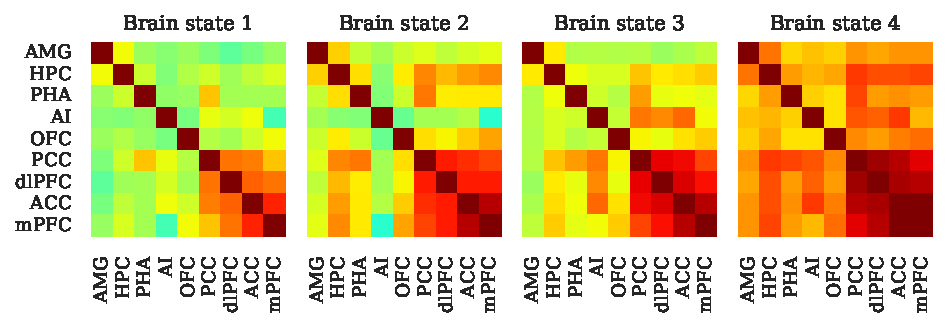
\includegraphics[width=\textwidth]{fig/ukbiobank/brain_states/self_reported_depression_state_brain_states_SVWP_joint_k04}}
  \caption{
    UK Biobank extracted brain states, separately for each cohort stratification.
  }\label{fig:ukb-results-brain-states}
\end{figure}


The corresponding dwell times are shown in \cref{fig:ukb-results-brain-states-dwell-times-dlo,fig:ukb-results-brain-states-dwell-times-srlo,fig:ukb-results-brain-states-dwell-times-srds}.
For both lifetime occurrence analyses, participants in the depressed cohorts spend significantly (two-sample $t$-test) \emph{more} time in state~1 (Cohen~$d = 0.16$, $p = .004$; Cohen~$d = 0.10$, $p = .04$, respectively) and \emph{less} time in state~2 (Cohen~$d = 0.17$, $p = .002$; Cohen~$d = 0.11$, $p = .03$).
However, for the self-reported depressed state analysis, while participants also spend significantly more time in state~1 (Cohen~$d = 0.12$, $p = .001$), they spend significantly less time in state~3 instead (Cohen~$d = 0.09$, $p = .02$).

These findings can partially be explained by the global reduced connectivity effect (i.e.~depressed participants spend less time in the lower connectivity strength brain state).
However, the lifetime occurrence depressed cohorts spending less time in a state with strong hippocampal-prefrontal connectivity could indicate lifetime changes or in-born differences related to the \gls{hpc}, potentially as a result of said depressive episodes and/or any received treatment.
The \gls{hpc} is involved with memory, and prefrontal areas are known to regulate such processes.
A weaker coupling between these regions could therefore be related to rumination, a cardinal depressive symptom.
%
The depressed \emph{state} cohort participants spending less time in a state with stronger insular-prefrontal connectivity could signal a more momentarily, active disturbance in emotional processing, regulation of homeostasis and (para)sympathetic stress management.


\begin{figure}[ht]
  \centering
  \subcaptionbox{Diagnosed lifetime occurrence\label{fig:ukb-results-brain-states-dwell-times-dlo}}{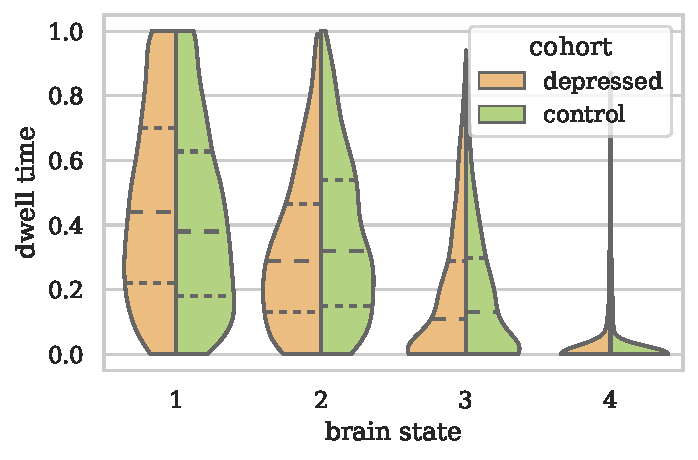
\includegraphics[width=0.6\textwidth]{fig/ukbiobank/brain_states/diagnosed_lifetime_occurrence_brain_states_SVWP_joint_k04_dwell_times}}
  \subcaptionbox{Self-reported lifetime occurrence\label{fig:ukb-results-brain-states-dwell-times-srlo}}{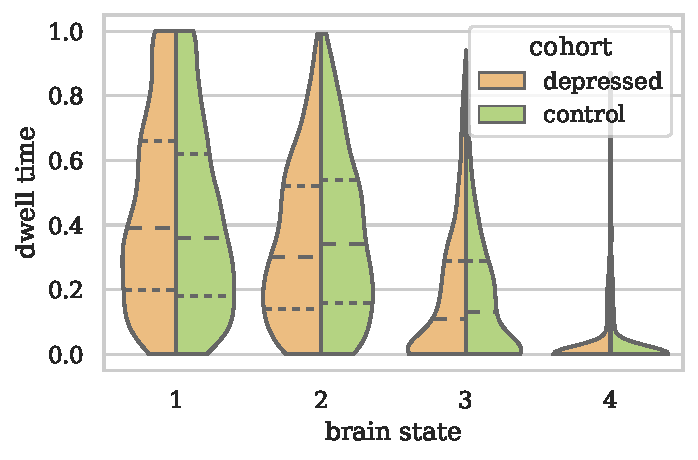
\includegraphics[width=0.6\textwidth]{fig/ukbiobank/brain_states/lifetime_occurrence_brain_states_SVWP_joint_k04_dwell_times}}
  \subcaptionbox{Self-reported depressed state\label{fig:ukb-results-brain-states-dwell-times-srds}}{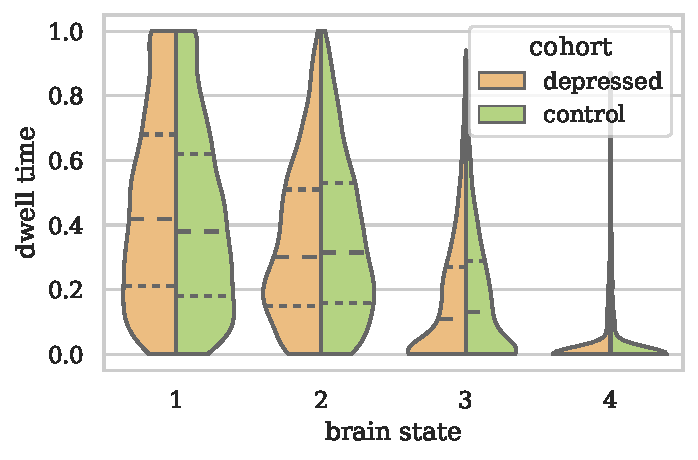
\includegraphics[width=0.6\textwidth]{fig/ukbiobank/brain_states/self_reported_depression_state_brain_states_SVWP_joint_k04_dwell_times}}
  \caption{
    UK Biobank brain state dwell times, separately extracted and computed for each cohort stratification.
  }\label{fig:ukb-results-brain-states-dwell-times}
\end{figure}


None of the switch rates between cohorts differ significantly.
